\chapter{Introducción}
\label{cap:capitulo1}
\setcounter{page}{1}

\begin{flushright}
\begin{minipage}[]{10cm}
\emph{El éxito es la capacidad de ir de fracaso en fracaso sin perder el entusiasmo.}\\
\end{minipage}\\

Winston Churchill\\
\end{flushright}
\vspace{2cm}
\noindent En la actualidad, los robots desempeñan un papel fundamental en el ámbito educativo, tanto en institutos como en universidades. Su 
incorporación ha demostrado ser muy beneficiosa para el desarrollo de habilidades \acs{STEM} y la enseñanza del pensamiento computacional 
entre los estudiantes. No obstante, es esencial que estos robots no tengan un coste elevado, permitiendo así que las escuelas puedan hacerse 
con una cantidad significativa de ellos. De esta forma, cada alumno tendría la oportunidad de disfrutar de un aprendizaje enriquecedor e individualizado.

El presente trabajo se centra en el desarrollo de un robot industrial de tamaño reducido y bajo coste, diseñado con el propósito de 
facilitar su uso y control. Este robot ha sido completamente impreso en 3D y se encuentra integrado con herramientas ampliamente 
utilizadas en el ámbito de la robótica. Esta combinación permite que cualquier estudiante tenga acceso a él y, al replicar el proyecto, 
aprenda de manera práctica sobre el apasionante mundo de la impresión 3D.

En este capítulo introductorio se abordará el contexto de la robótica, explorando sus diversas disciplinas y aplicaciones. Esto nos ayudará a 
comprender mejor el ámbito en el cual se enmarca este trabajo, proporcionando una base sólida para comprender los conceptos y desarrollos que 
se presentarán a lo largo del documento.

\newpage
\section{Robótica}
\label{sec:rob}
\noindent La robótica es la ciencia dedicada al diseño, construcción y programación de robots. Se entiende por 
robot a una máquina programable capaz de llevar a cabo tareas de forma autónoma, usando sensores para percibir su entorno y 
actuadores para interactuar con él.

Ya en la antigüedad se encuentran referencias a autómatas y dispositivos mecánicos  
que tratan de imitar acciones humanas. Sin embargo, no es hasta mediados del siglo XX cuando surge el concepto de robot tal y como lo conocemos hoy en día. 
En 1954, George Devol y Joseph Engelberger desarrollaron el primer robot industrial programable llamado \textit{Unimate} (Figura \ref{fig:unimate}), el cual fue utilizado en la fábrica General Motors 
para realizar tareas de soldadura en la línea de producción de automóviles. Este hito marcó el comienzo de la automatización industrial y sentó las bases para 
el desarrollo futuro de robots industriales.\\
\begin{figure} [ht!]
  \begin{center}
    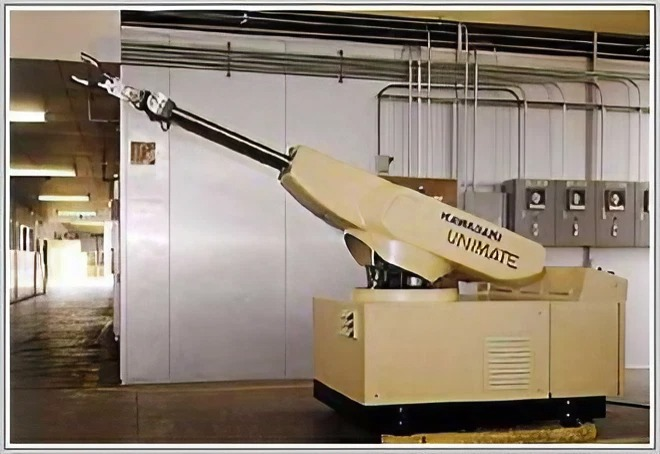
\includegraphics[width=7cm]{figs/unimate.jpg}
  \end{center}
  \caption{Robot Unimate}
  \label{fig:unimate}
\end{figure}\ 

En las décadas posteriores se produjeron numerosos avances en robótica; se desarrollaron robots cada vez más sofisticados que cubrían una amplia gama de tareas más allá de la 
automatización industrial. Un claro ejemplo de ello fue el robot \textit{Shakey} (Figura \ref{fig:shakey}), desarrollado por el laboratorio de investigación de la Universidad de Stanford en 1966. Se trataba 
de un robot cuyo único propósito era navegar autónomamente en una sala con obstáculos gracias al uso de sensores y algoritmos de planificación.\\
\begin{figure} [ht!]
  \begin{center}
    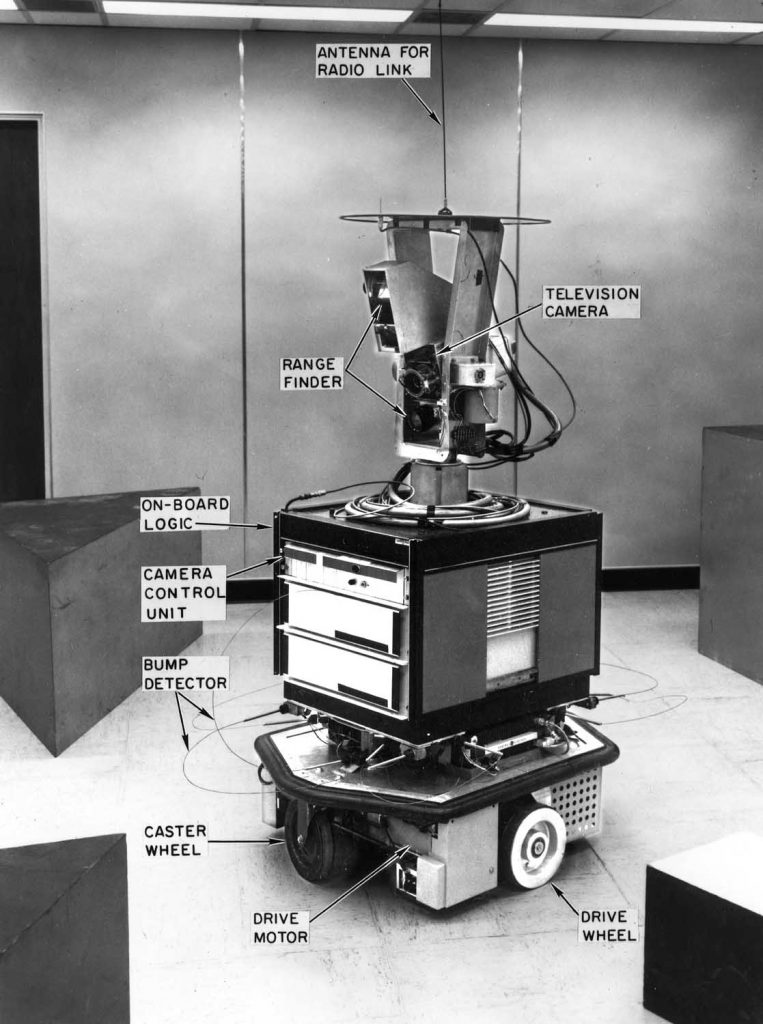
\includegraphics[width=7cm]{figs/shakey.jpg}
  \end{center}
  \caption{Robot Shakey}
  \label{fig:shakey}
\end{figure}\

En la década de 1970, el uso de robots industriales se había disparado en todo el mundo. Estos robots, conocidos como robots manipuladores, fueron utilizados para 
realizar todo tipo de tareas repetitivas y peligrosas en fábricas.
\\
\indent En las últimas décadas, la robótica ha seguido avanzando a pasos agigantados. Los avances en la capacidad de cómputo, el aprendizaje automático y la visión 
artificial han permitido el desarrollo de robots cada vez más inteligentes.
\\

\indent En la actualidad, la robótica está presente en numerosos sectores, abarcando una gran variedad de aplicaciones. Esta versatilidad ha llevado al surgimiento 
de diversos grupos y categorías que nos permiten clasificar las diferentes tipos de robots. Un claro ejemplo de ello es la robótica 
de servicio, que integra robots en aplicaciones cotidianas.
\newpage

\section{Robótica de servicio}
\noindent Un robot de servicio es un tipo de robot diseñado para realizar tareas en beneficio de los seres humanos. Estos robots están 
destinados a interactuar directamente con las personas, por lo que están equipados con gran variedad de sensores, actuadores y sistemas de 
inteligencia artificial, que les permiten percibir y comprender el entorno que los rodea. 
En función de su ámbito de uso, pueden llegar a realizar una amplia gama de tareas, como limpieza y mantenimiento del hogar, 
asistencia en la intervención médica, entrega de alimentos y productos, cuidado de personas mayores, entre otros. A continuación, 
veremos algunos ejemplos de estos robots.

\subsubsection{Robots de campo}
Se considera robot de campo a un robot diseñado para su uso en exteriores; lo que significa que trabajará bajo unas duras condiciones. 
Se trata de un sector heterogéneo en el cual se engloban los 
robots espaciales, agrícolas, búsqueda y rescate, inspección de instalaciones, minería, submarinos y conducción autónoma. En la Figura \ref{fig:campo} 
se muestran algunos ejemplos.
\begin{figure} [ht!]
  \centering    
  \subfigure[NASA Opportunity]{\label{fig:opportunity}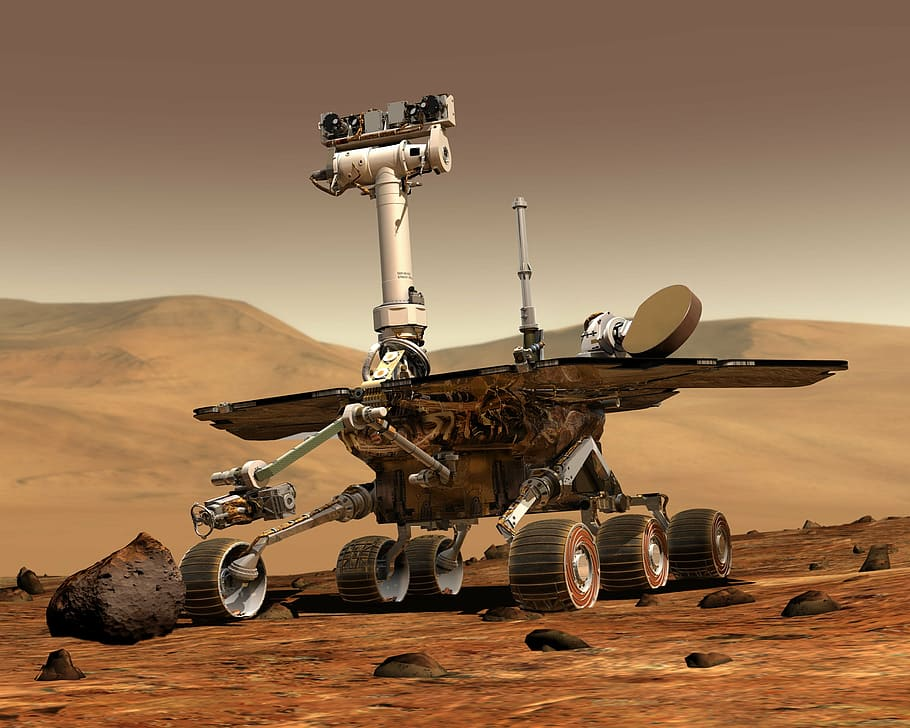
\includegraphics[width=0.3\linewidth ]{figs/rover.jpg}}
  \hspace{3cm}
  \subfigure[Tractor autónomo]{\label{fig:roomba_agua}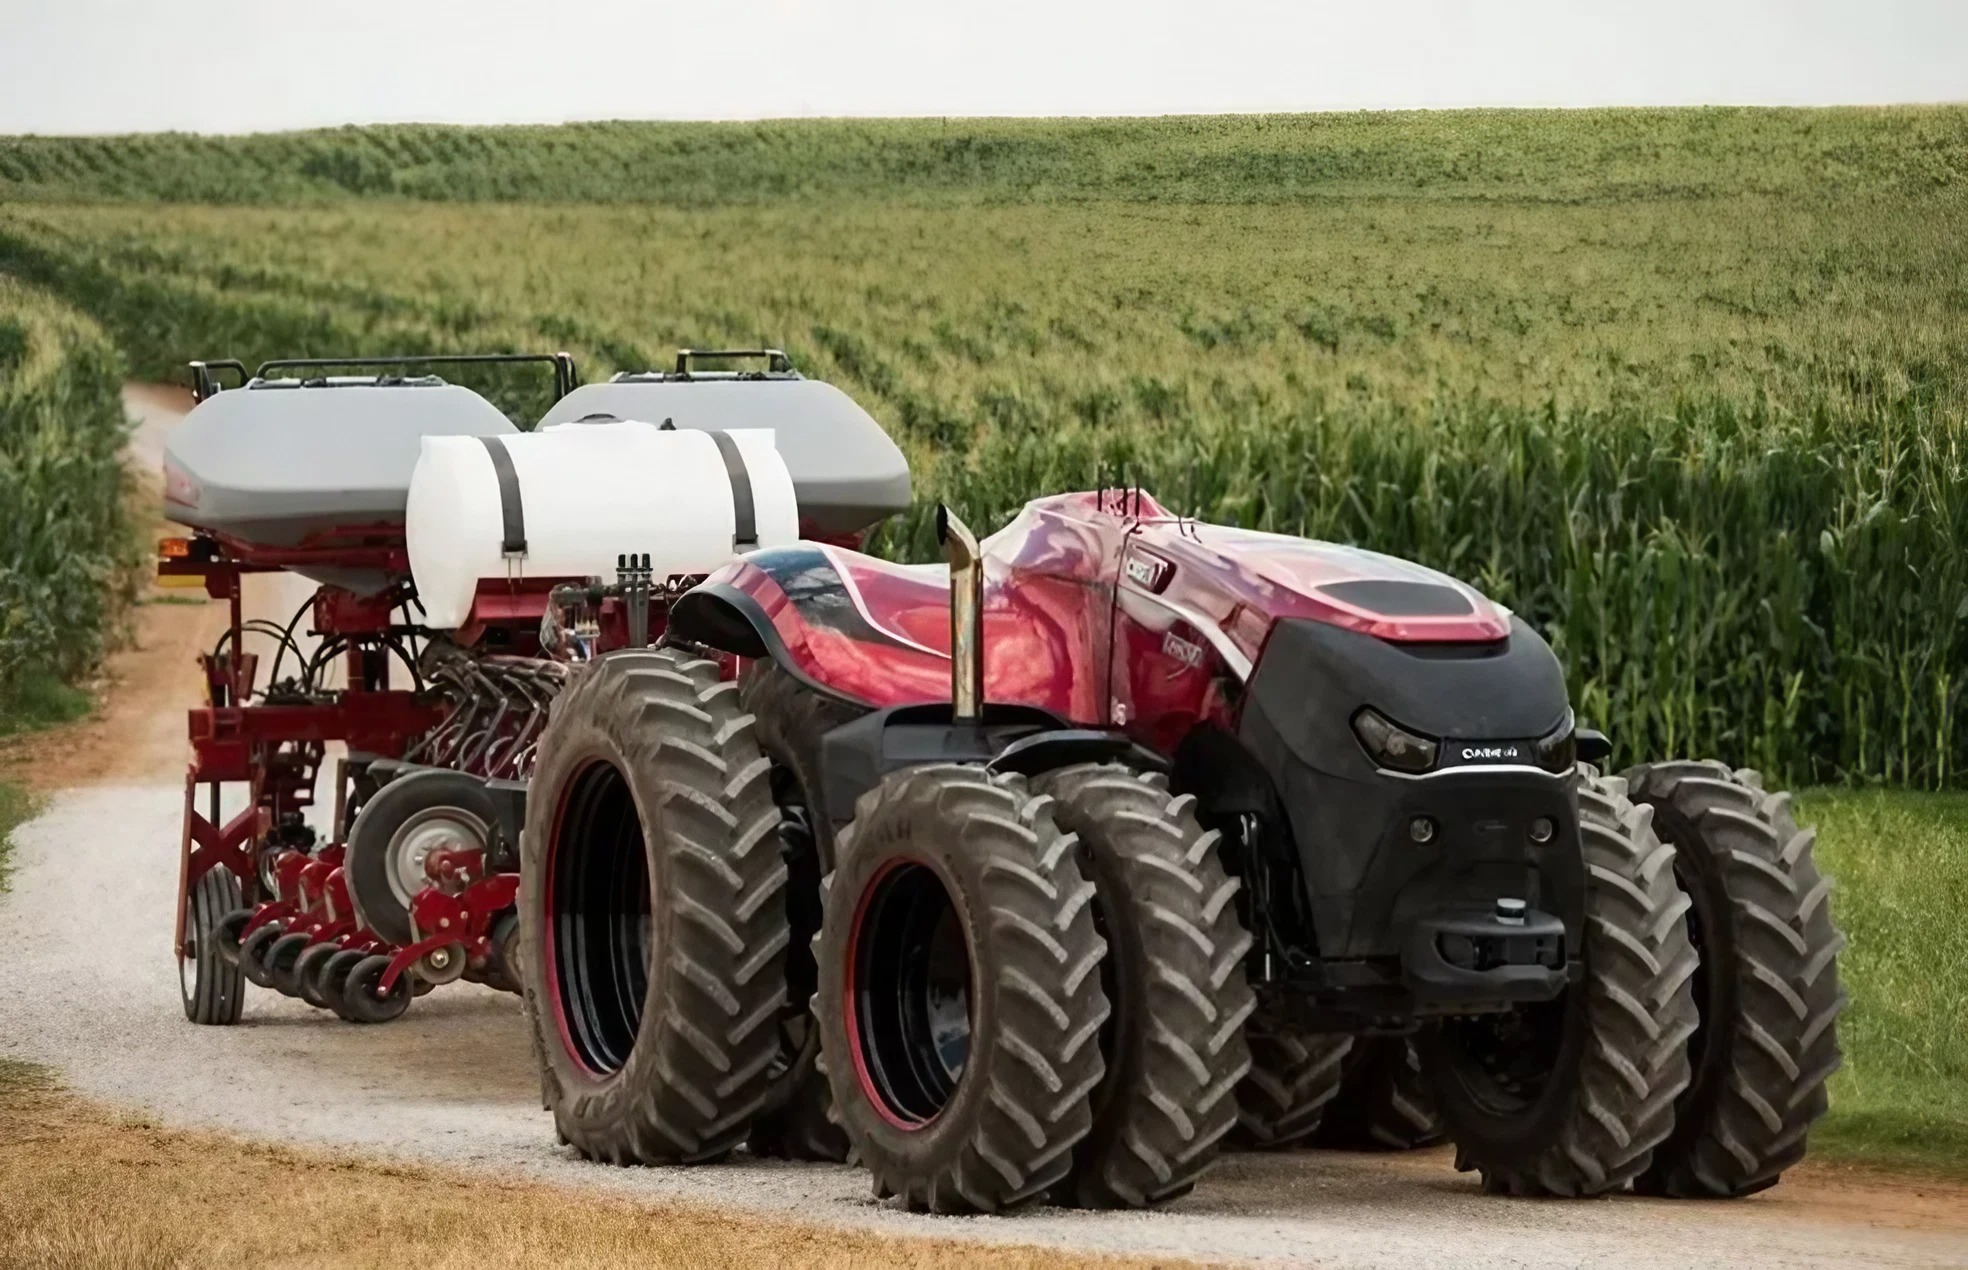
\includegraphics[width=0.3\linewidth]{figs/tractor.jpg}}
  \hspace{3cm}
  \subfigure[ROV Victor 6000]{\label{fig:rov}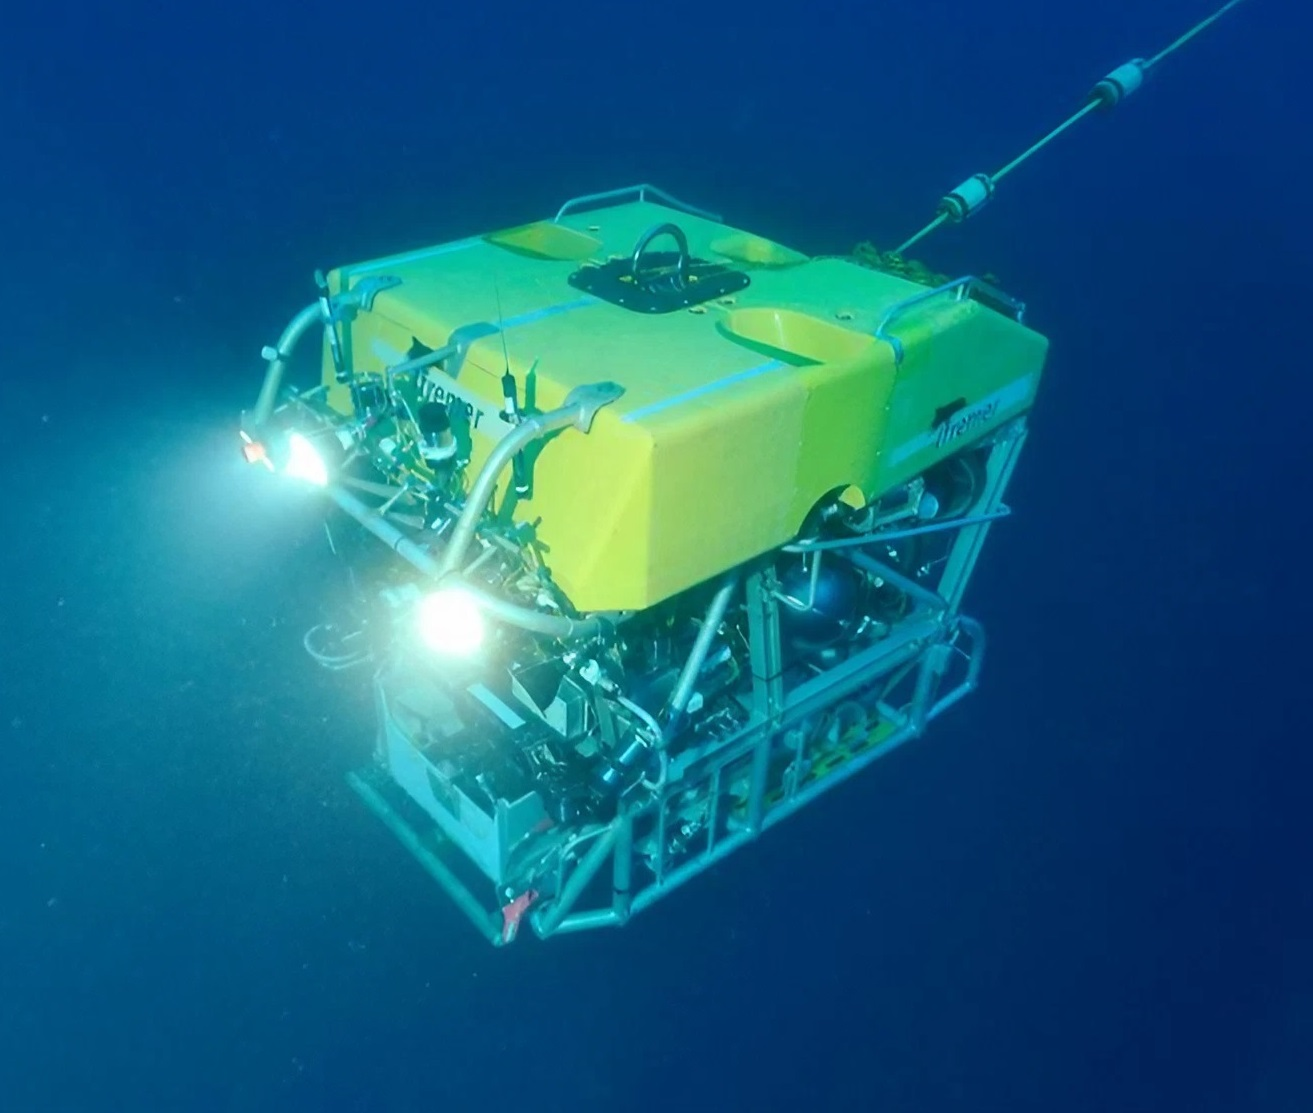
\includegraphics[width=0.3\linewidth]{figs/rov.jpg}}
  \hspace{3cm}
  \subfigure[Boston Dynamics Spot]{\label{fig:spot}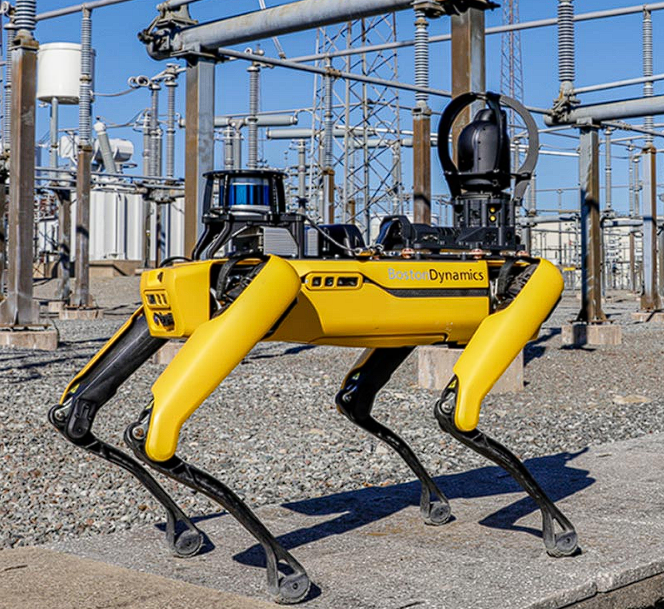
\includegraphics[width=0.3\linewidth]{figs/spot.png}}
  \caption{Robots de campo}
  \label{fig:campo}
\end{figure}
\newpage
\subsubsection{Robots de limpieza}
Son aquellos robots creados para eliminar la suciedad en hogares y empresas. En función de sus características, pueden ser usados para aspirar y fregar el suelo, o incluso,
para limpiar los cristales exteriores de los edificios. Se trata de una tecnología asentada y robusta que a día de hoy cuenta con más de 20 años en el mercado. Pese a esto, 
se pueden encontrar diferentes categorías de robot en función de las necesidades. En la actualidad, integran cada vez más sensores para realizar una limpieza más eficaz y 
en entornos más imprevisibles (cables, animales, objetos tirados, etc). En la Figura \ref{fig:limpieza} se muestran algunos de los más usados.

\begin{figure} [ht!]
  \centering    
  \subfigure[Roomba J7+]{\label{fig:roomba}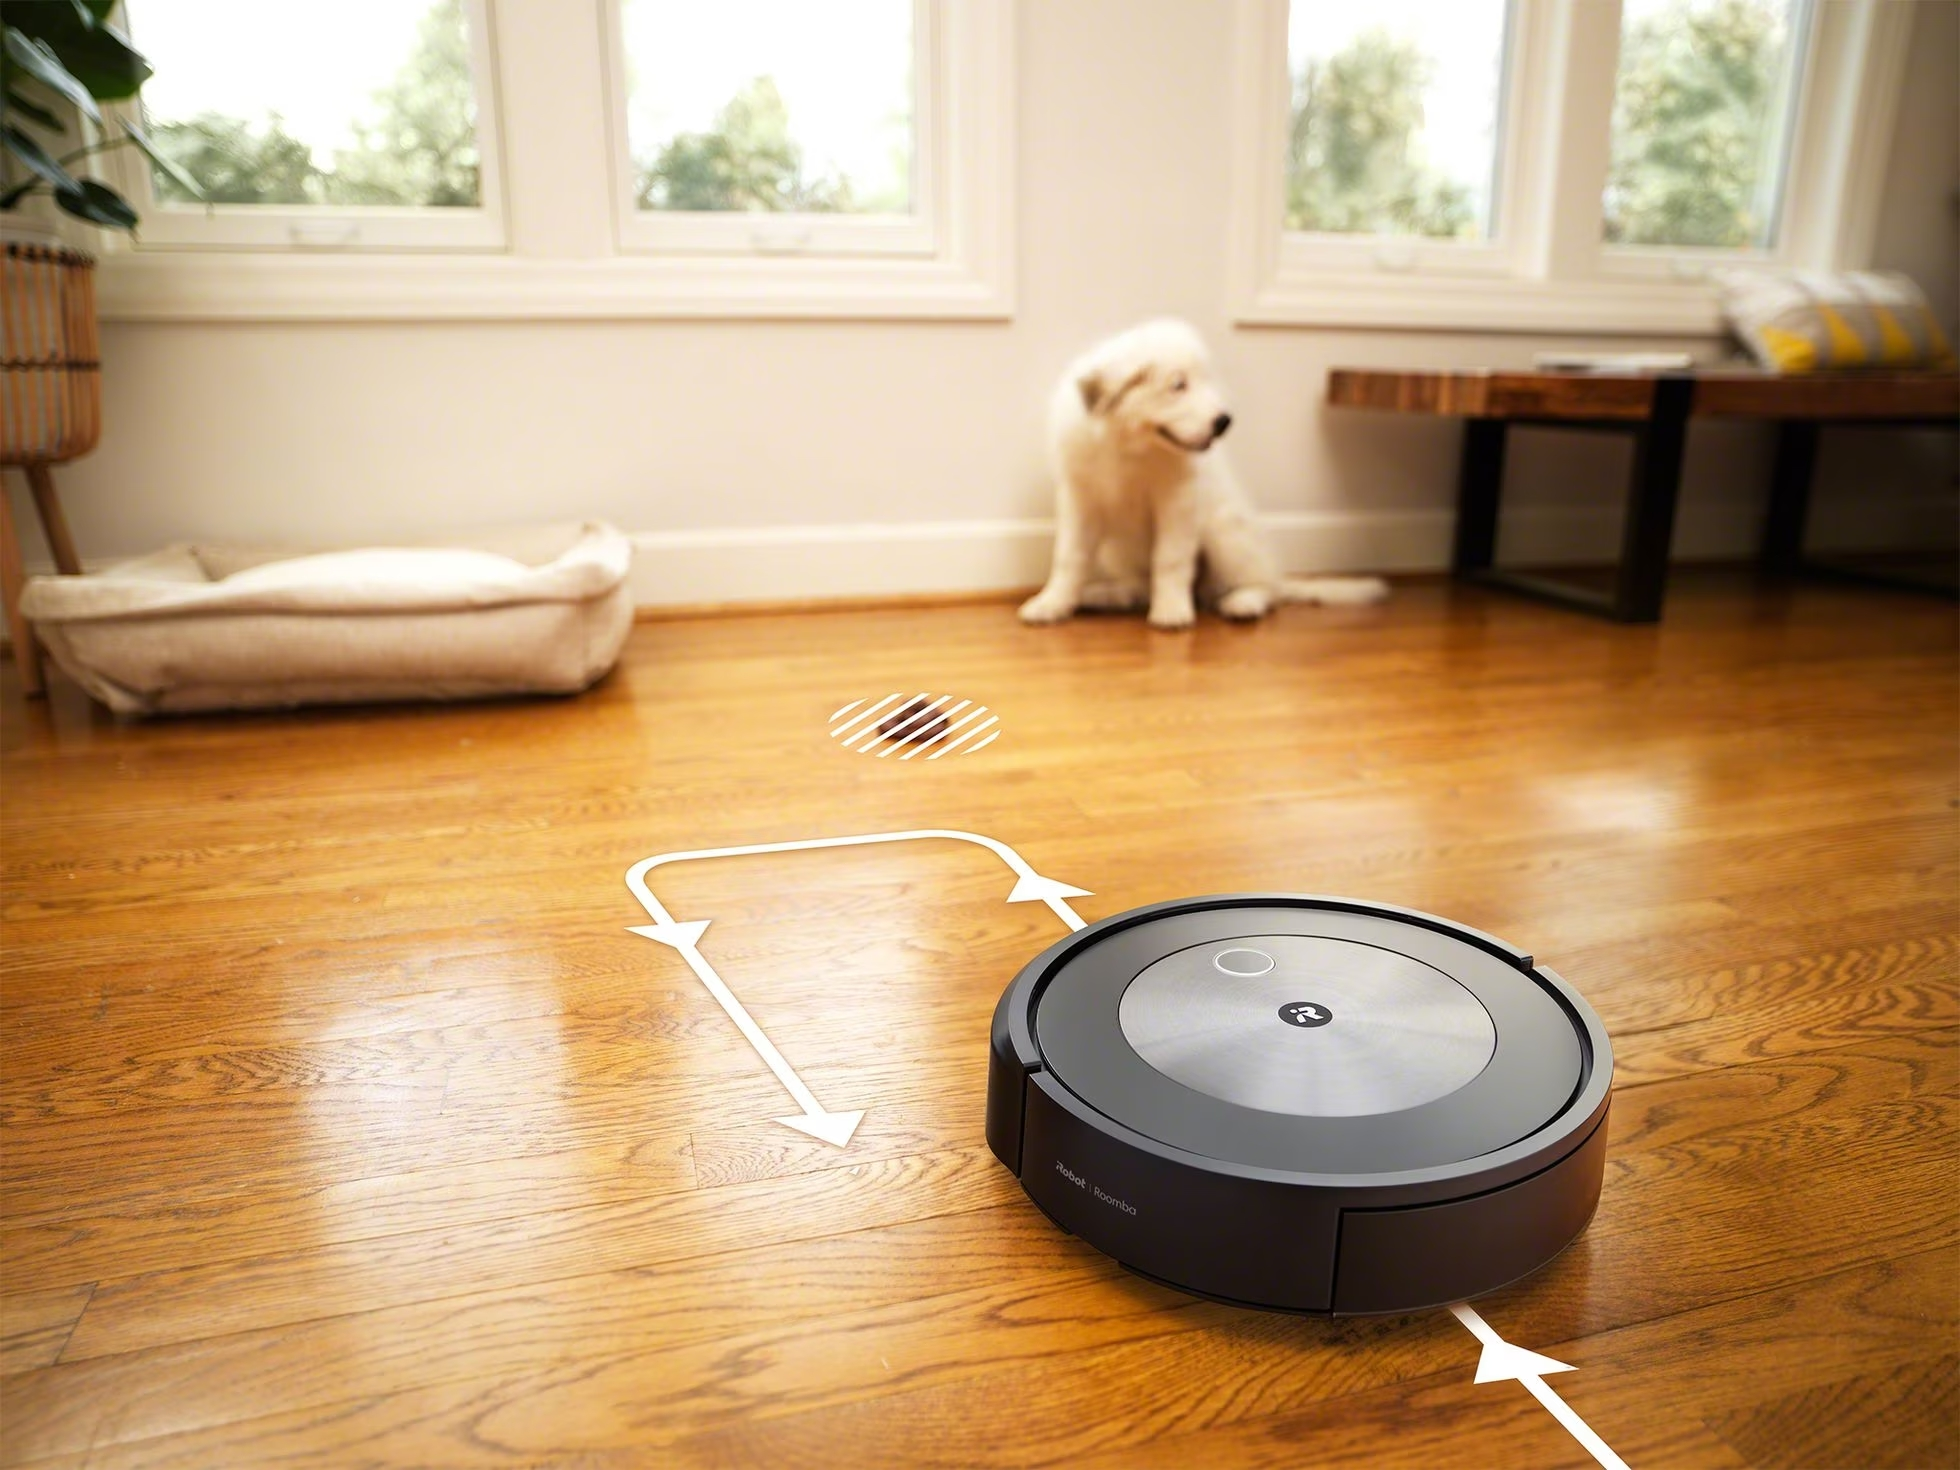
\includegraphics[width=0.25\linewidth ]{figs/roomba.jpg}}
  \hspace{1cm}
  \subfigure[Roomba Braava]{\label{fig:roomba_agua}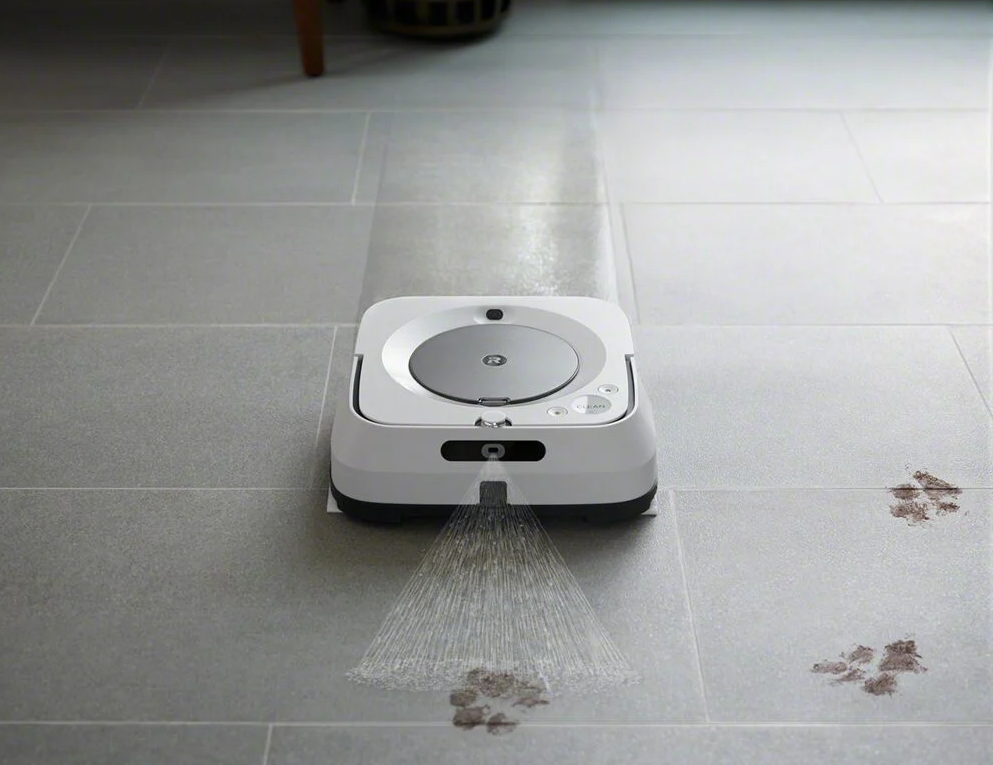
\includegraphics[width=0.25\linewidth]{figs/roombaAgua.jpg}}
  \hspace{1cm}
  \subfigure[Hobot 388]{\label{fig:hobot}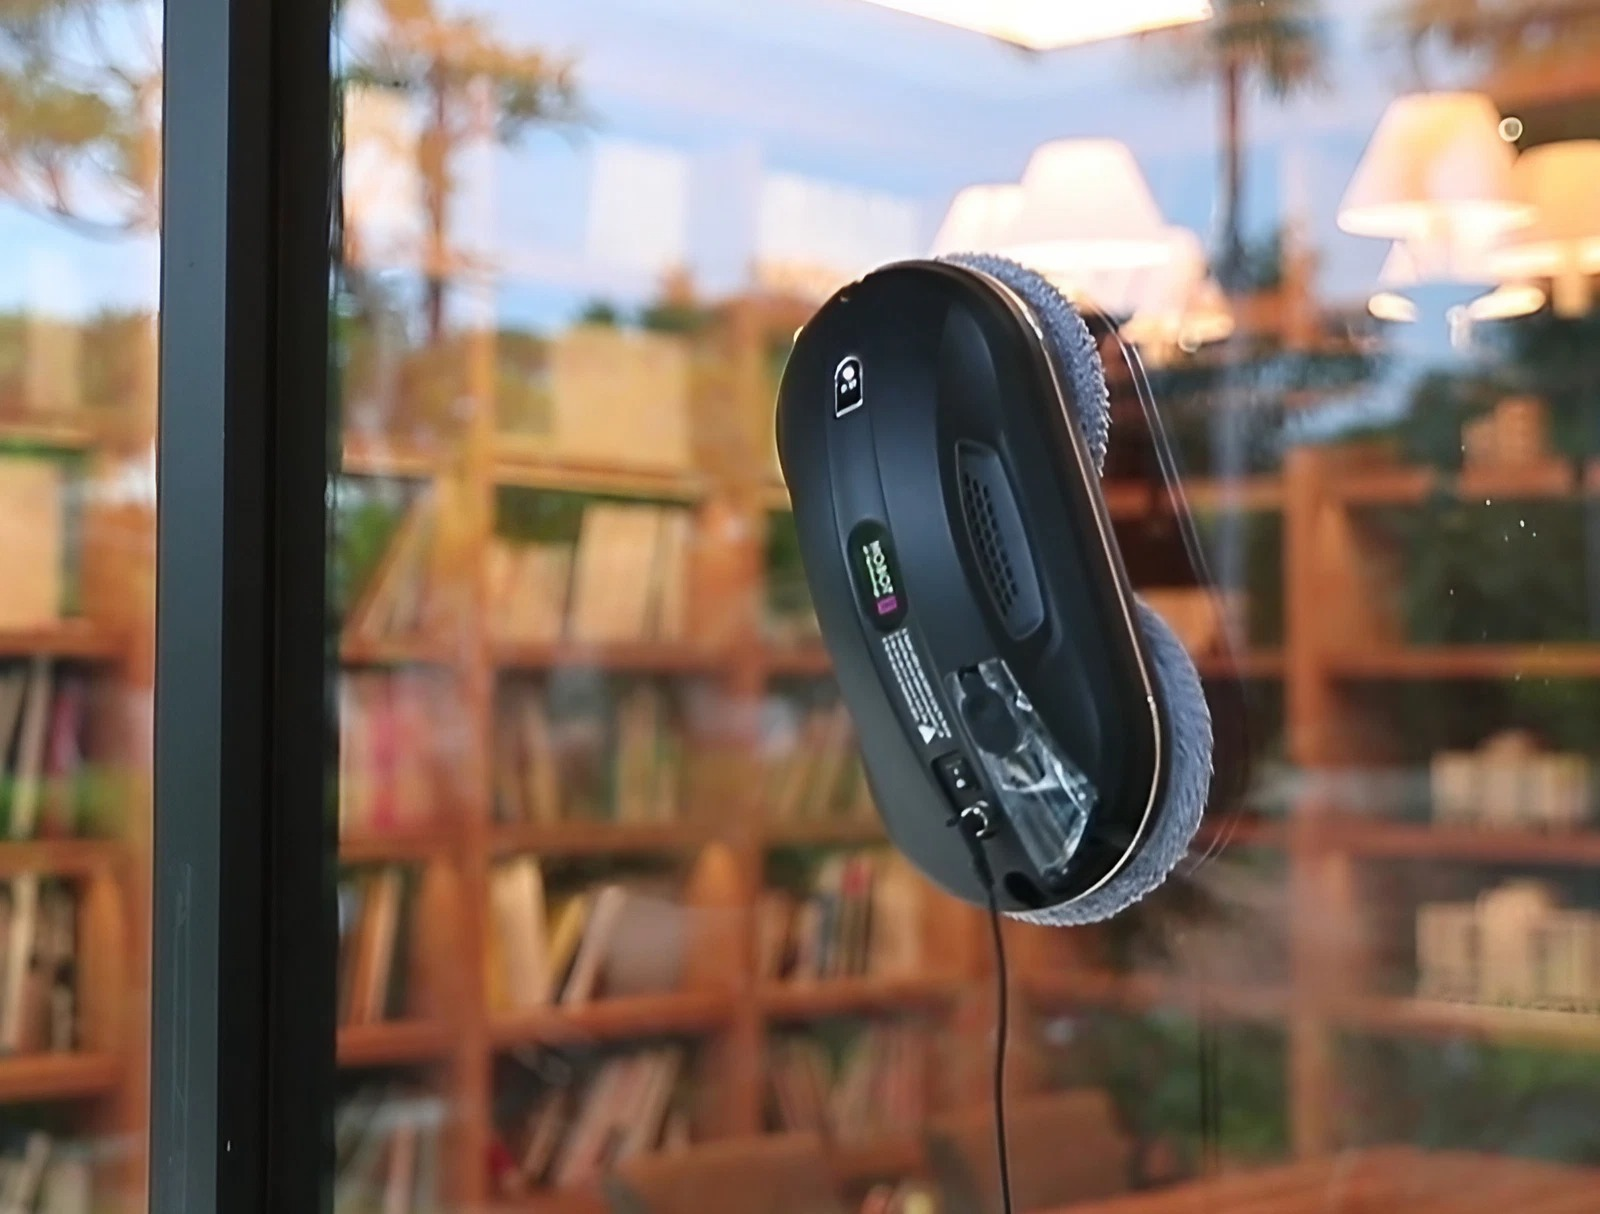
\includegraphics[width=0.25\linewidth]{figs/hobot.jpg}}
  \caption{Robots de limpieza}
  \label{fig:limpieza}
\end{figure}

\subsubsection{Robots de entretenimiento}
Los robots de entretenimiento son máquinas diseñadas para proporcionar diversión y compañía a las personas. Están equipados con capacidades y 
características específicas que los hacen adecuados para interactuar con las personas. Tienen una apariencia amigable y agradable, como los mostrados 
en la Figura \ref{fig:entretenimiento}. Están pensados para 
evitar el efecto del \textit{Valle Inquietante}. Esta teoría sugiere que a medida que los robots se vuelven más humanos en apariencia y comportamiento, la respuesta 
emocional de las personas hacia ellos es más negativa, antes de volver a ser positiva a medida que se vuelven prácticamente 
indistinguibles de los seres humanos reales.
\begin{figure} [ht!]
  \centering    
  \subfigure[Aibo Sony]{\label{fig:aibo}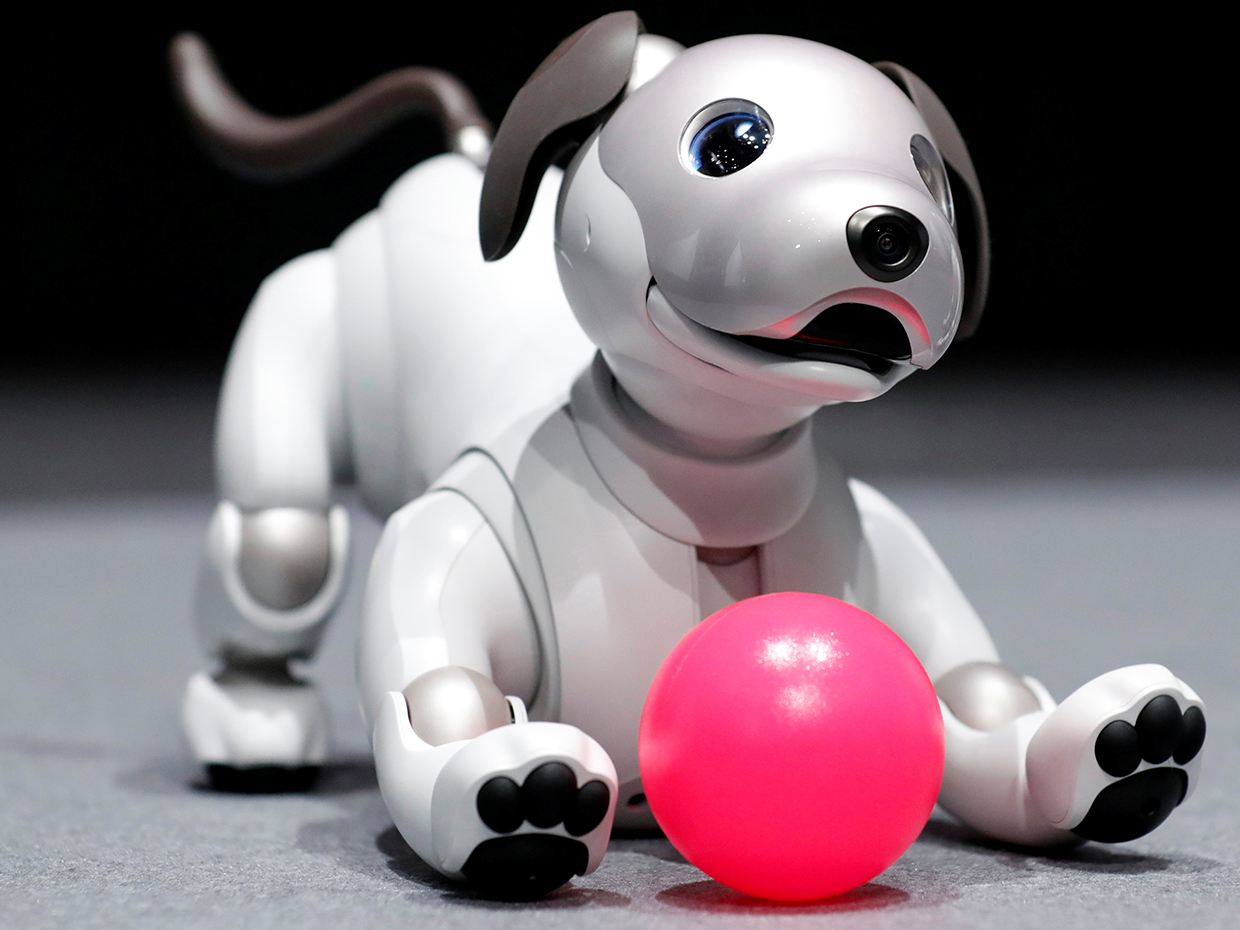
\includegraphics[width=0.28\linewidth ]{figs/aibo.jpeg}}
  \hspace{1cm}
  \subfigure[Foca Paro]{\label{fig:paro}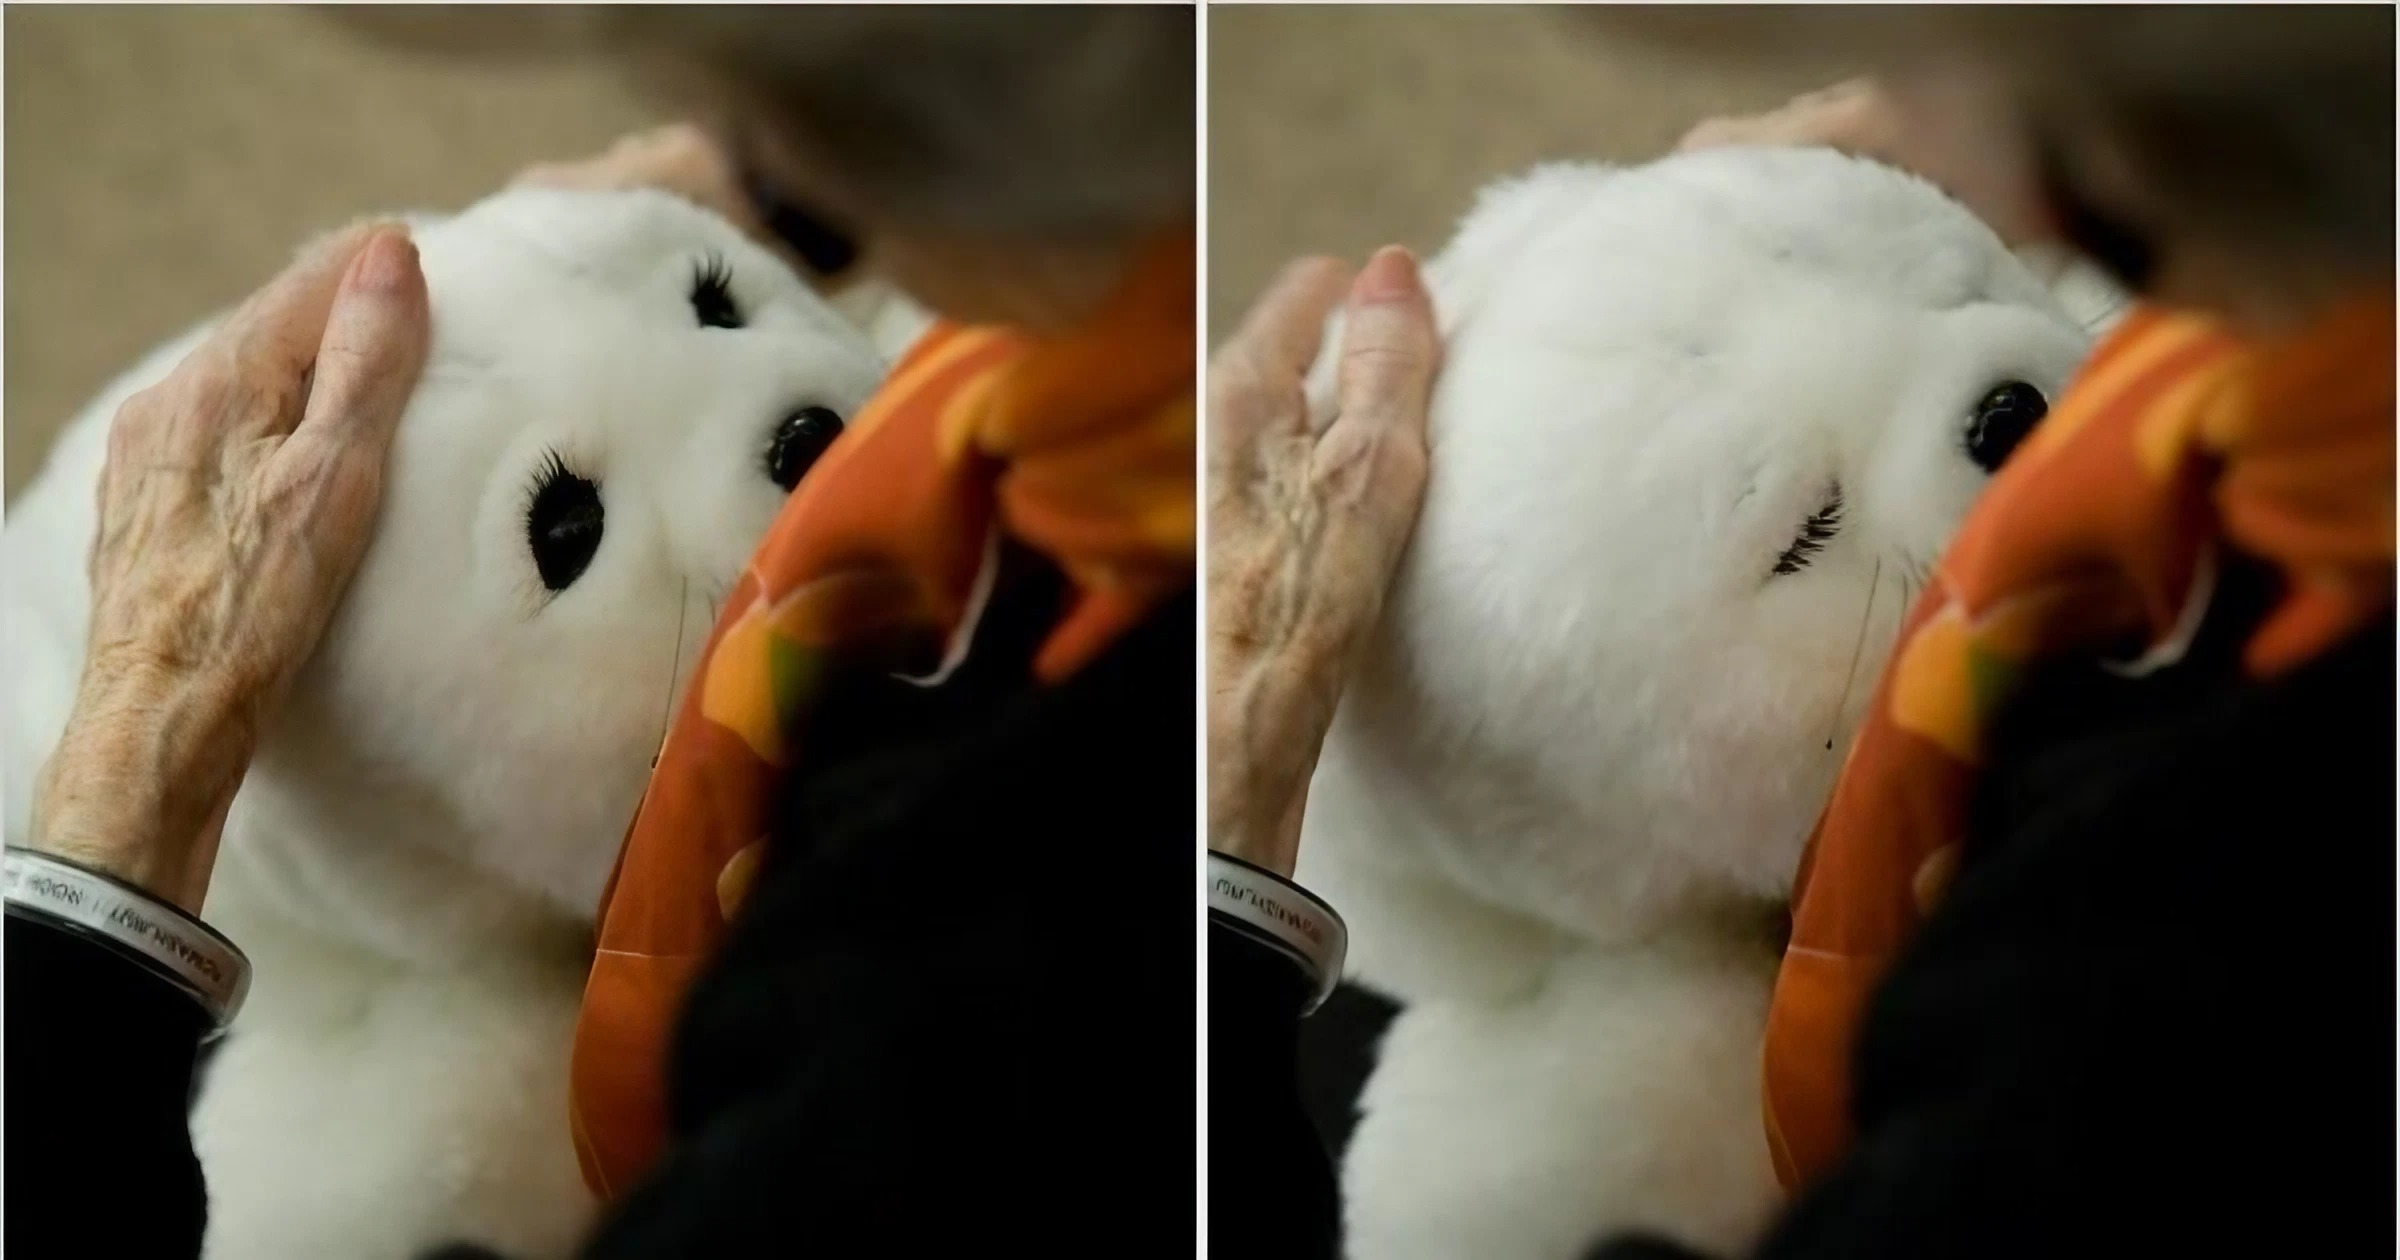
\includegraphics[width=0.4\linewidth]{figs/paro.jpeg}}
  \caption{Robots de entretenimiento}
  \label{fig:entretenimiento}
\end{figure}

\subsubsection{Robots en salud}
Los robots en el campo de la salud están diseñados para proporcionar ayuda en entornos médicos y de atención sanitaria. Desempeñan tareas 
variadas como pueden ser la cirugía (Figura \ref{fig:davinci}), la rehabilitación (Figura \ref{fig:rehabilitacion}) y la trasferencia de pacientes (Figura \ref{fig:trasferencia}), entre otros.

\begin{figure} [ht!]
  \centering    
  \subfigure[Da Vinci]{\label{fig:davinci}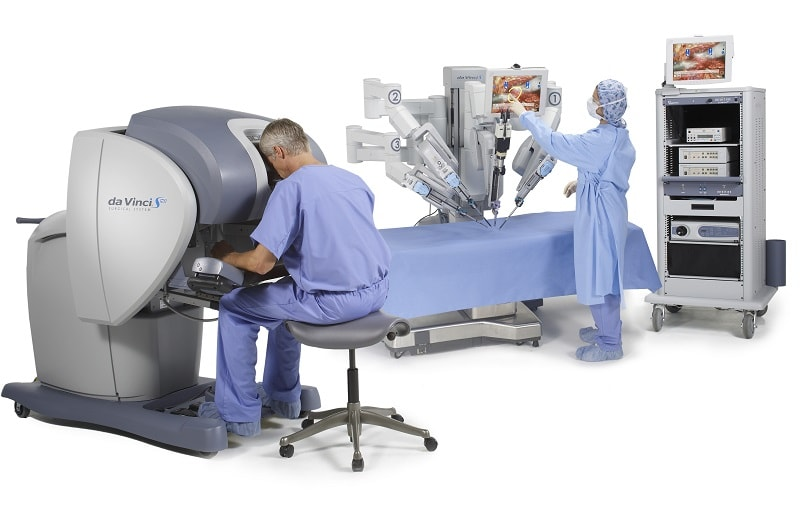
\includegraphics[width=0.25\linewidth ]{figs/davinci.jpg}}
  \hspace{0.5cm}
  \subfigure[Atlas Marsi Bionics]{\label{fig:rehabilitacion}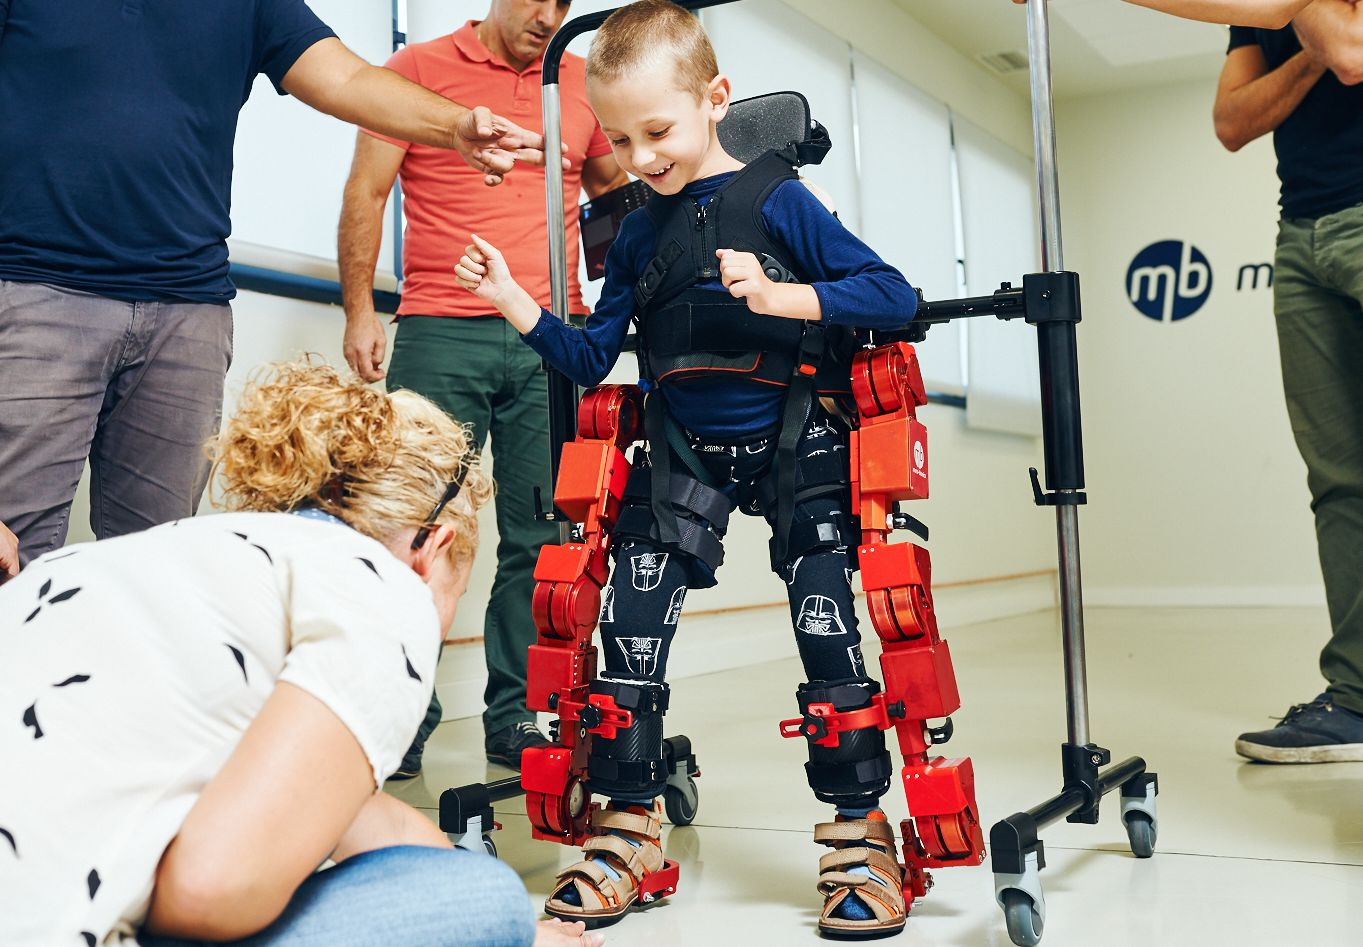
\includegraphics[width=0.25\linewidth]{figs/rehabilitacion.jpg}}
  \hspace{0.5cm}
  \subfigure[Riba 2]{\label{fig:trasferencia}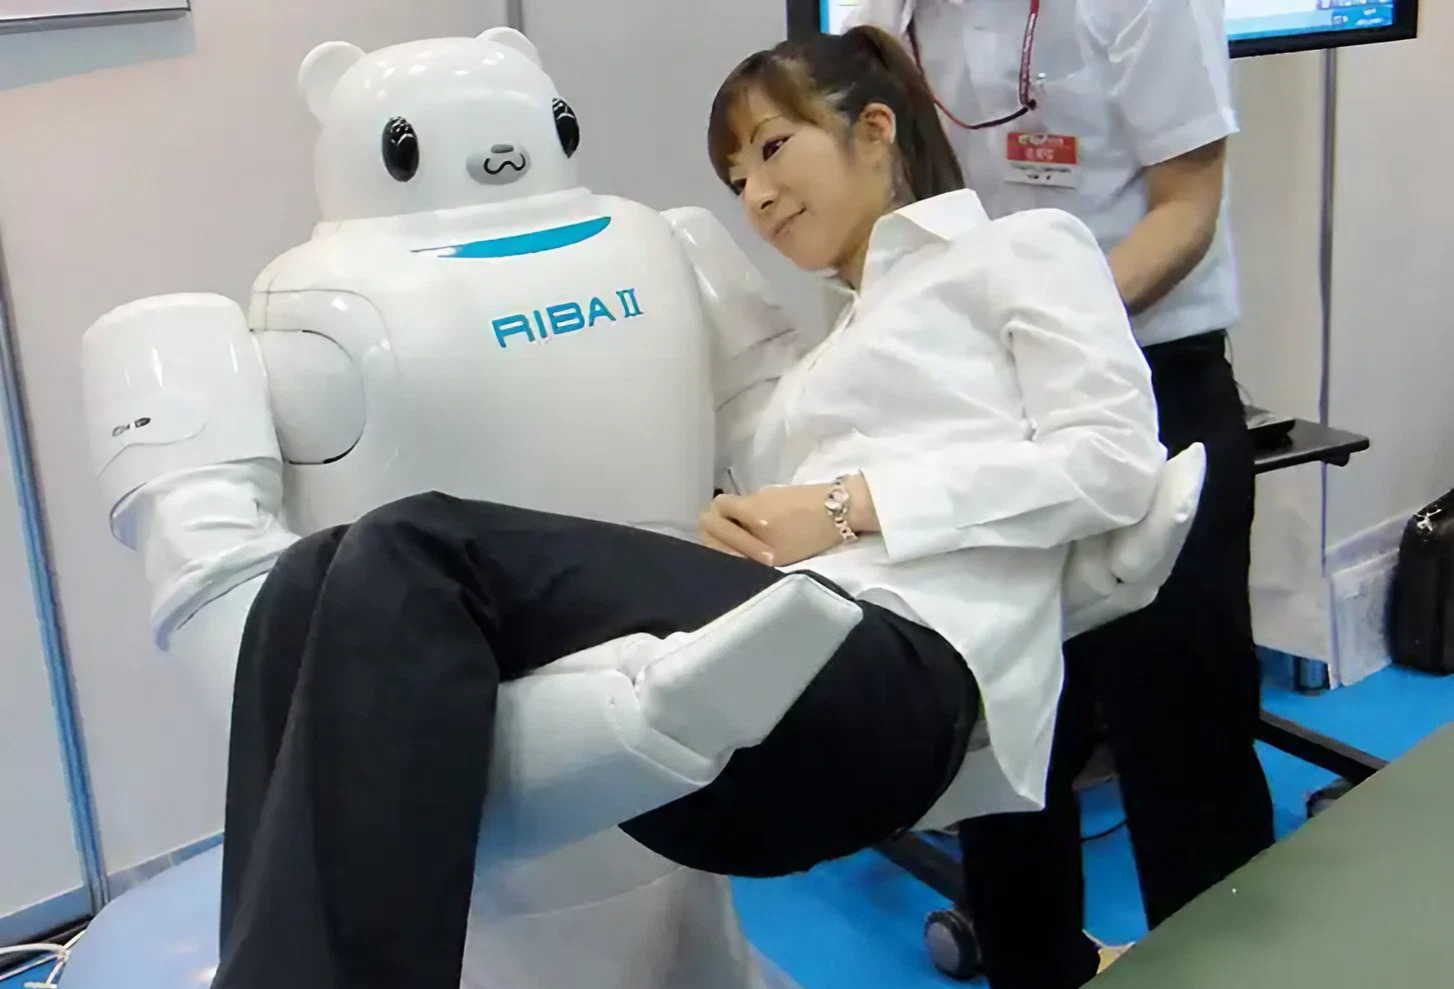
\includegraphics[width=0.25\linewidth]{figs/trasferencia.jpg}}
  \caption{Robots en el campo de la salud}
\end{figure}

\subsubsection{Robots en logística}
Los robots de logística están enfocados a tareas de transporte y organización de mercancías en almacenes y centros de distribución. 
Son capaces de moverse de manera autónoma, cargar y descargar objetos ágilmente y bajo demanda optimizando los procesos logísticos. Un ejemplo 
claro de ellos son los robots utilizados en Amazon (Figura \ref{fig:amr}).

Más allá de su uso de almacenes, cabe destacar los llamados robots de "última milla". Son aquellos usados en el reparto de comida y 
paquetes en las ciudades. Aunque actualmente se encuentra en fase de desarrollo, ya han sido probados algunos 
prototipos como el usado por Glovo en Londres para repartir comida (Figura \ref{fig:glovo})

\begin{figure} [ht!]
    \centering    
    \subfigure[AMR Amazon Robotics]{\label{fig:amr}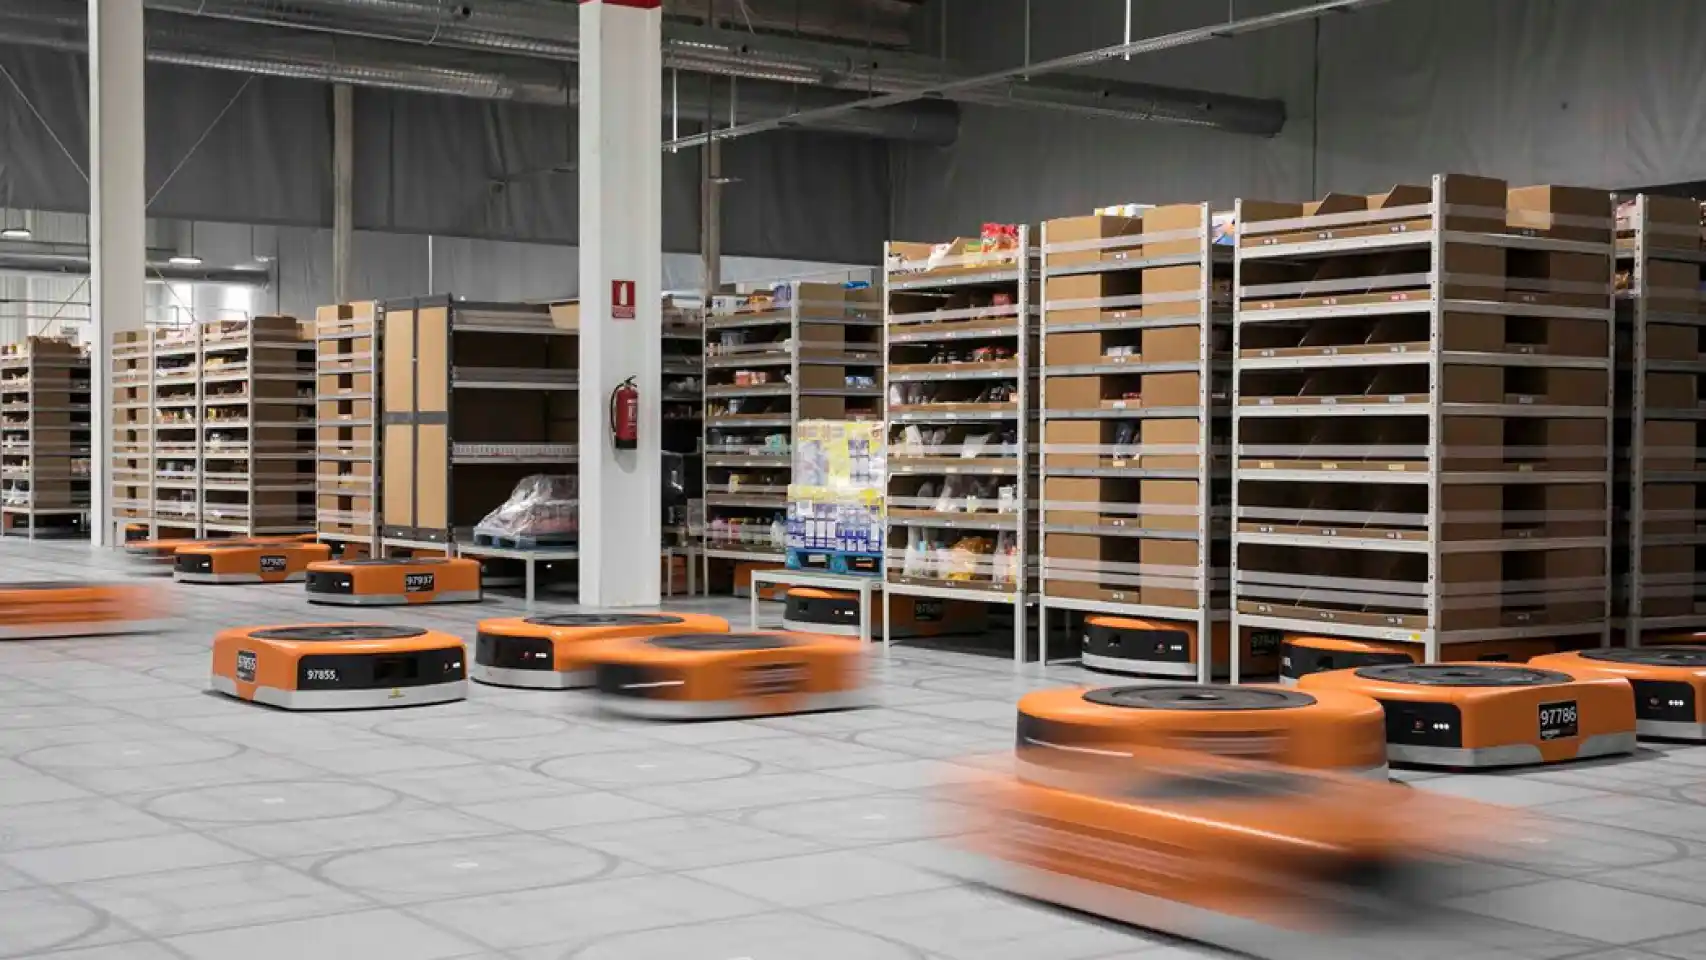
\includegraphics[width=0.4\linewidth]{figs/amr.jpg}}
    \hspace{1cm}
    \subfigure[Robot de reparto de Glovo]{\label{fig:glovo}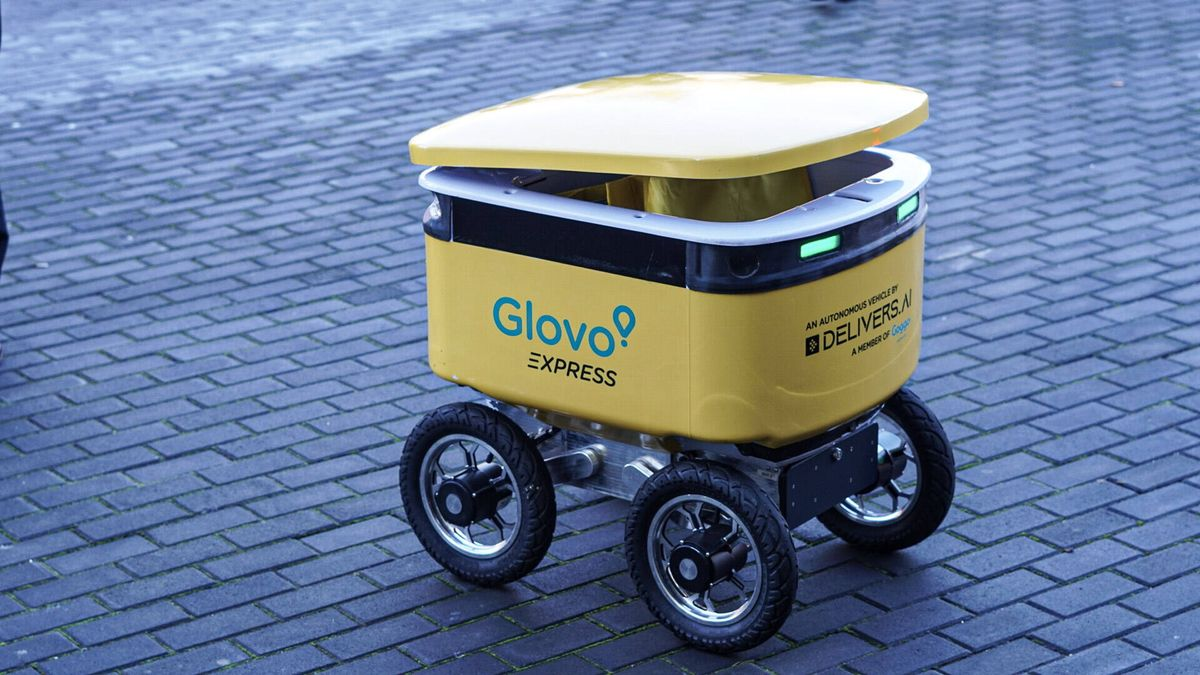
\includegraphics[width=0.4\linewidth]{figs/reparto.jpg}}

    \caption{Robots de logística}
\end{figure}


\newpage
\section{Robótica industrial}
\label{sec:rob_industrial}
\noindent Se entiende por robot industrial a una máquina automatizada diseñada específicamente para llevar a cabo tareas en entornos industriales. 
Disponen de numerosas articulaciones y una gran capacidad de maniobrabilidad. Su objetivo principal es reemplazar a un 
operario humano en tareas aburridas, sucias, peligrosas y exigentes (\textit{4D: Dull, Dirty, Dangerous and Demanding}).
En función de el número de articulaciones y la geometría del manipulador, se pueden clasificar en diferentes categorías.

\subsubsection{SCARA}
\label{sec:scara}
Los robots de tipo \acs{SCARA} se caracterizan por la disposición de sus 3, o 4, articulaciones con todos los ejes de rotación perpendiculares al suelo. Su capacidad para 
realizar movimientos rápidos y precisos en un plano horizontal lo hacen ideal para su uso en aplicaciones de ensamblaje electrónico, operaciones de 
\textit{pick and place} (coger componentes y situarlos) y empaquetado de productos, entre otras.
\begin{figure} [h!]
  \centering    
  \subfigure[Ensamblado de baterías]{\label{fig:fanuc}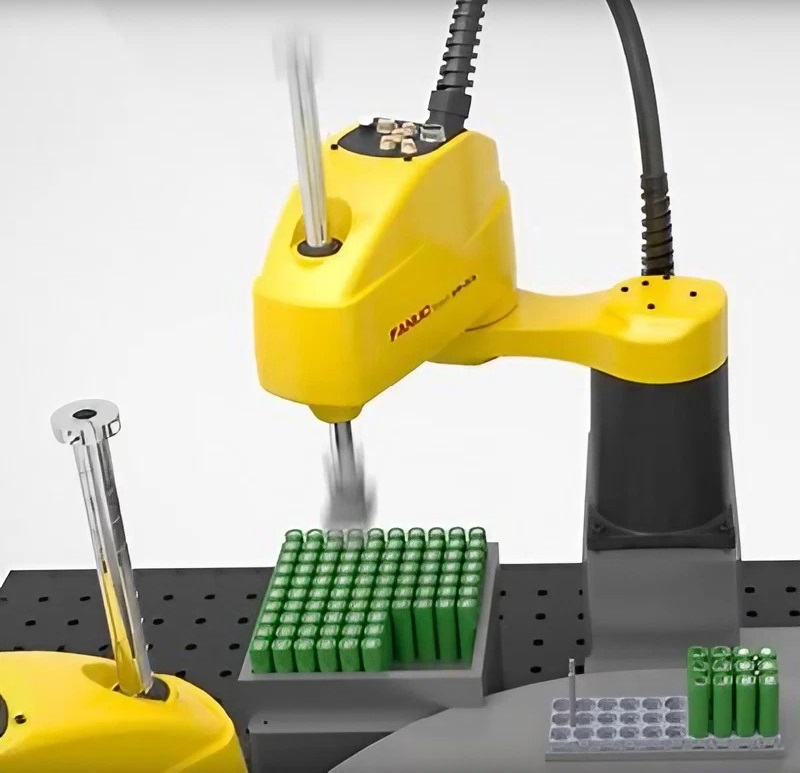
\includegraphics[width=0.3\linewidth ]{figs/fanuc.jpg}}
  \hspace{3cm}
  \subfigure[Espacio de trabajo]{\label{fig:fanuc_ws}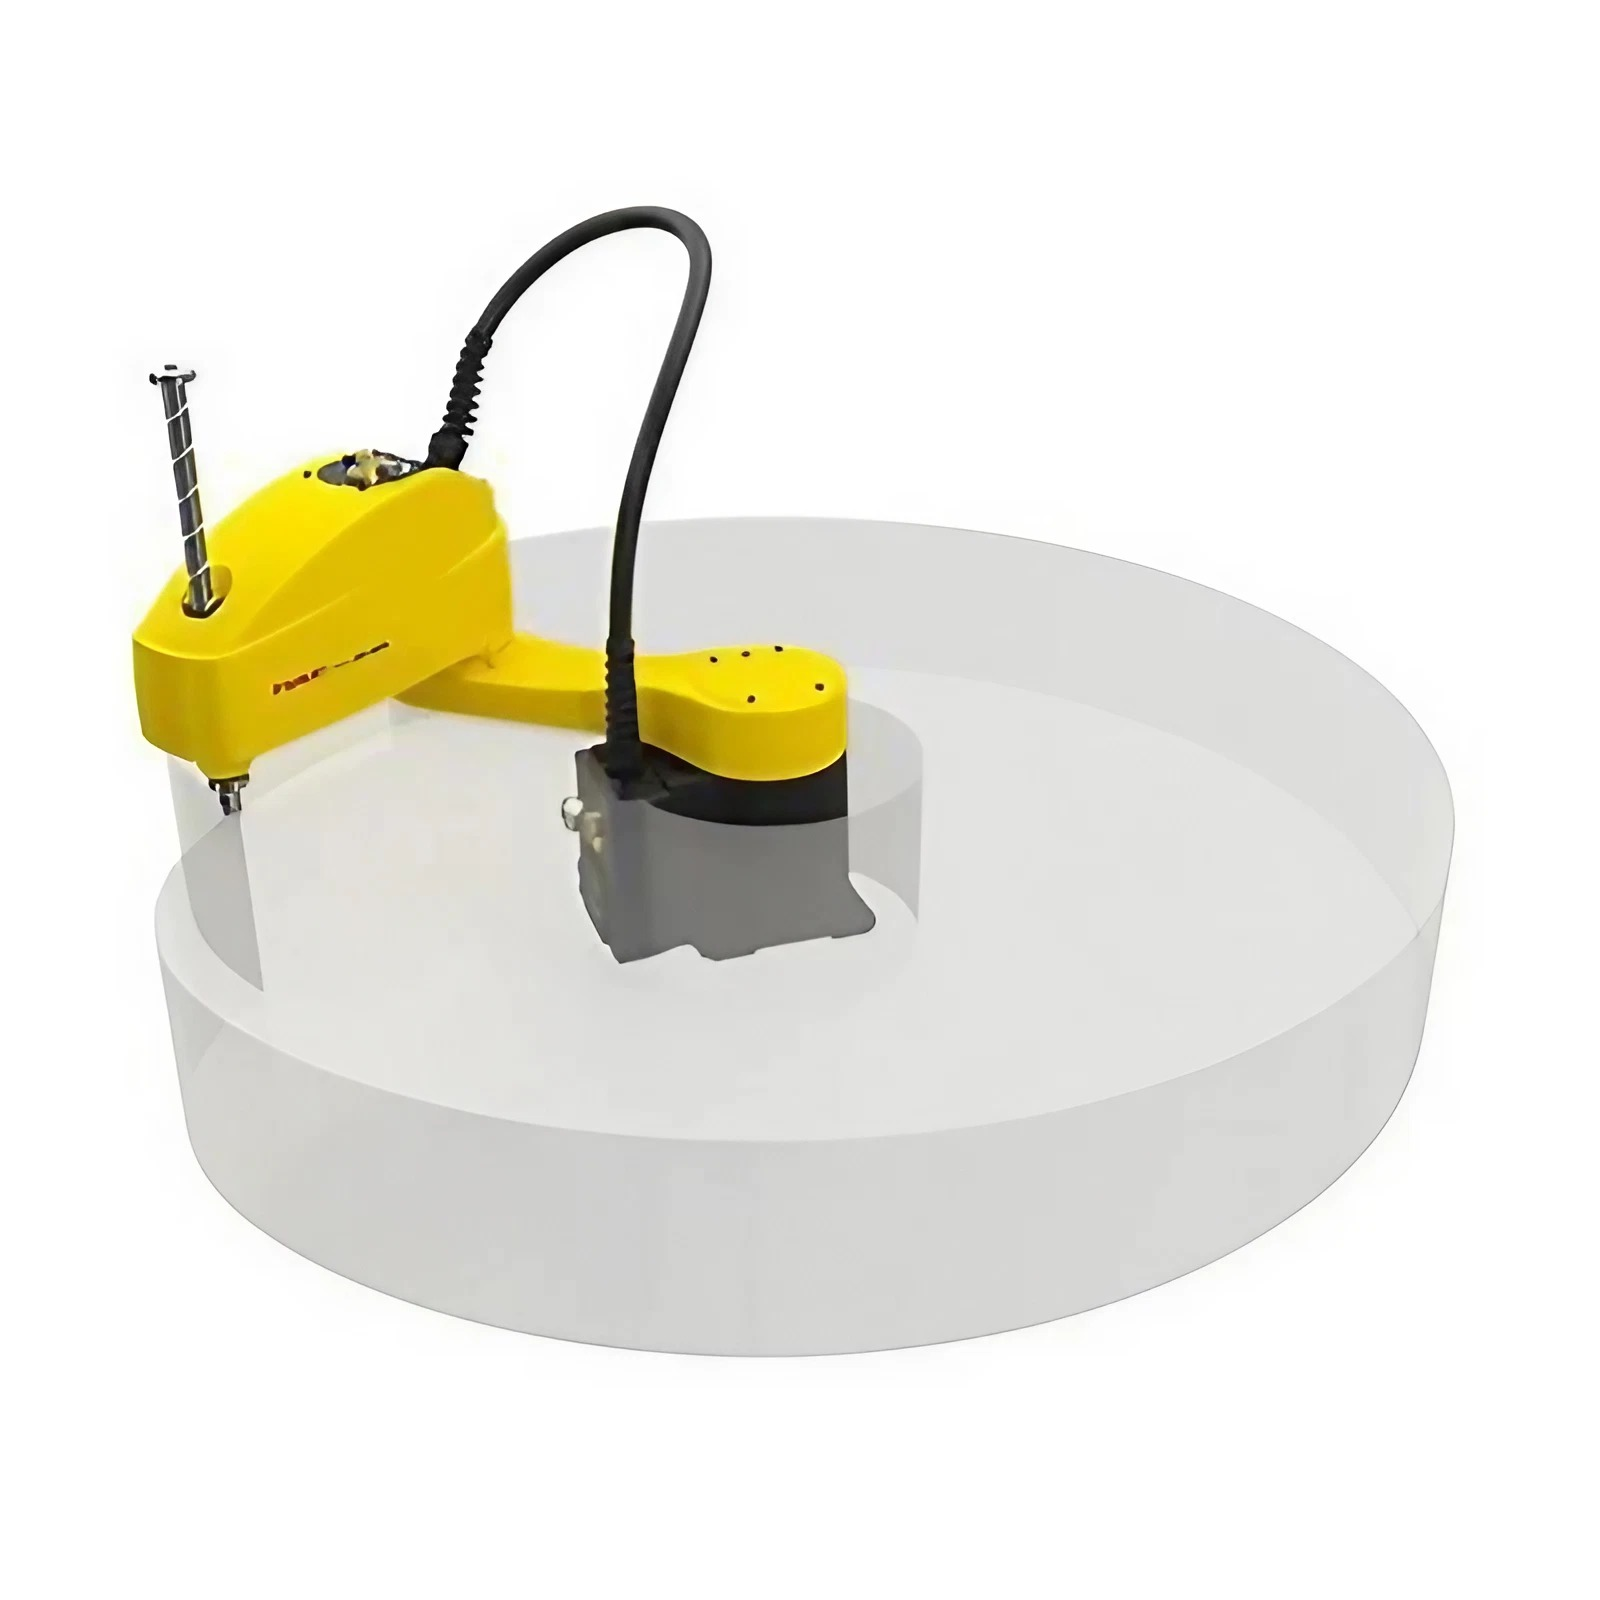
\includegraphics[width=0.4\linewidth]{figs/fanuc_spacio.jpg}}
  \caption[Fanuc SR-3iA]{Ejemplo: FANUC SR-3iA \footnote{\url{https://www.fanuc.eu/uk/en/robots/robot-filter-page/scara-series/scara-sr-3ia}}}
\end{figure}
\newpage
\subsubsection{Articulados}
Es el tipo de brazo robótico más usado en la industria. Están formados por una estructura similar a la de un brazo humano. Poseen entre 4 y 6 articulaciones de tipo 
revolución (giran en torno a un eje) permitiendo realizar movimientos complejos. 
\begin{figure} [h!]
  \centering    
  \subfigure[KUKA IONTEC \footnote{\url{https://www.kuka.com/es-es/productos-servicios/sistemas-de-robot/robot-industrial/kr-iontec}}]{\label{fig:iontec}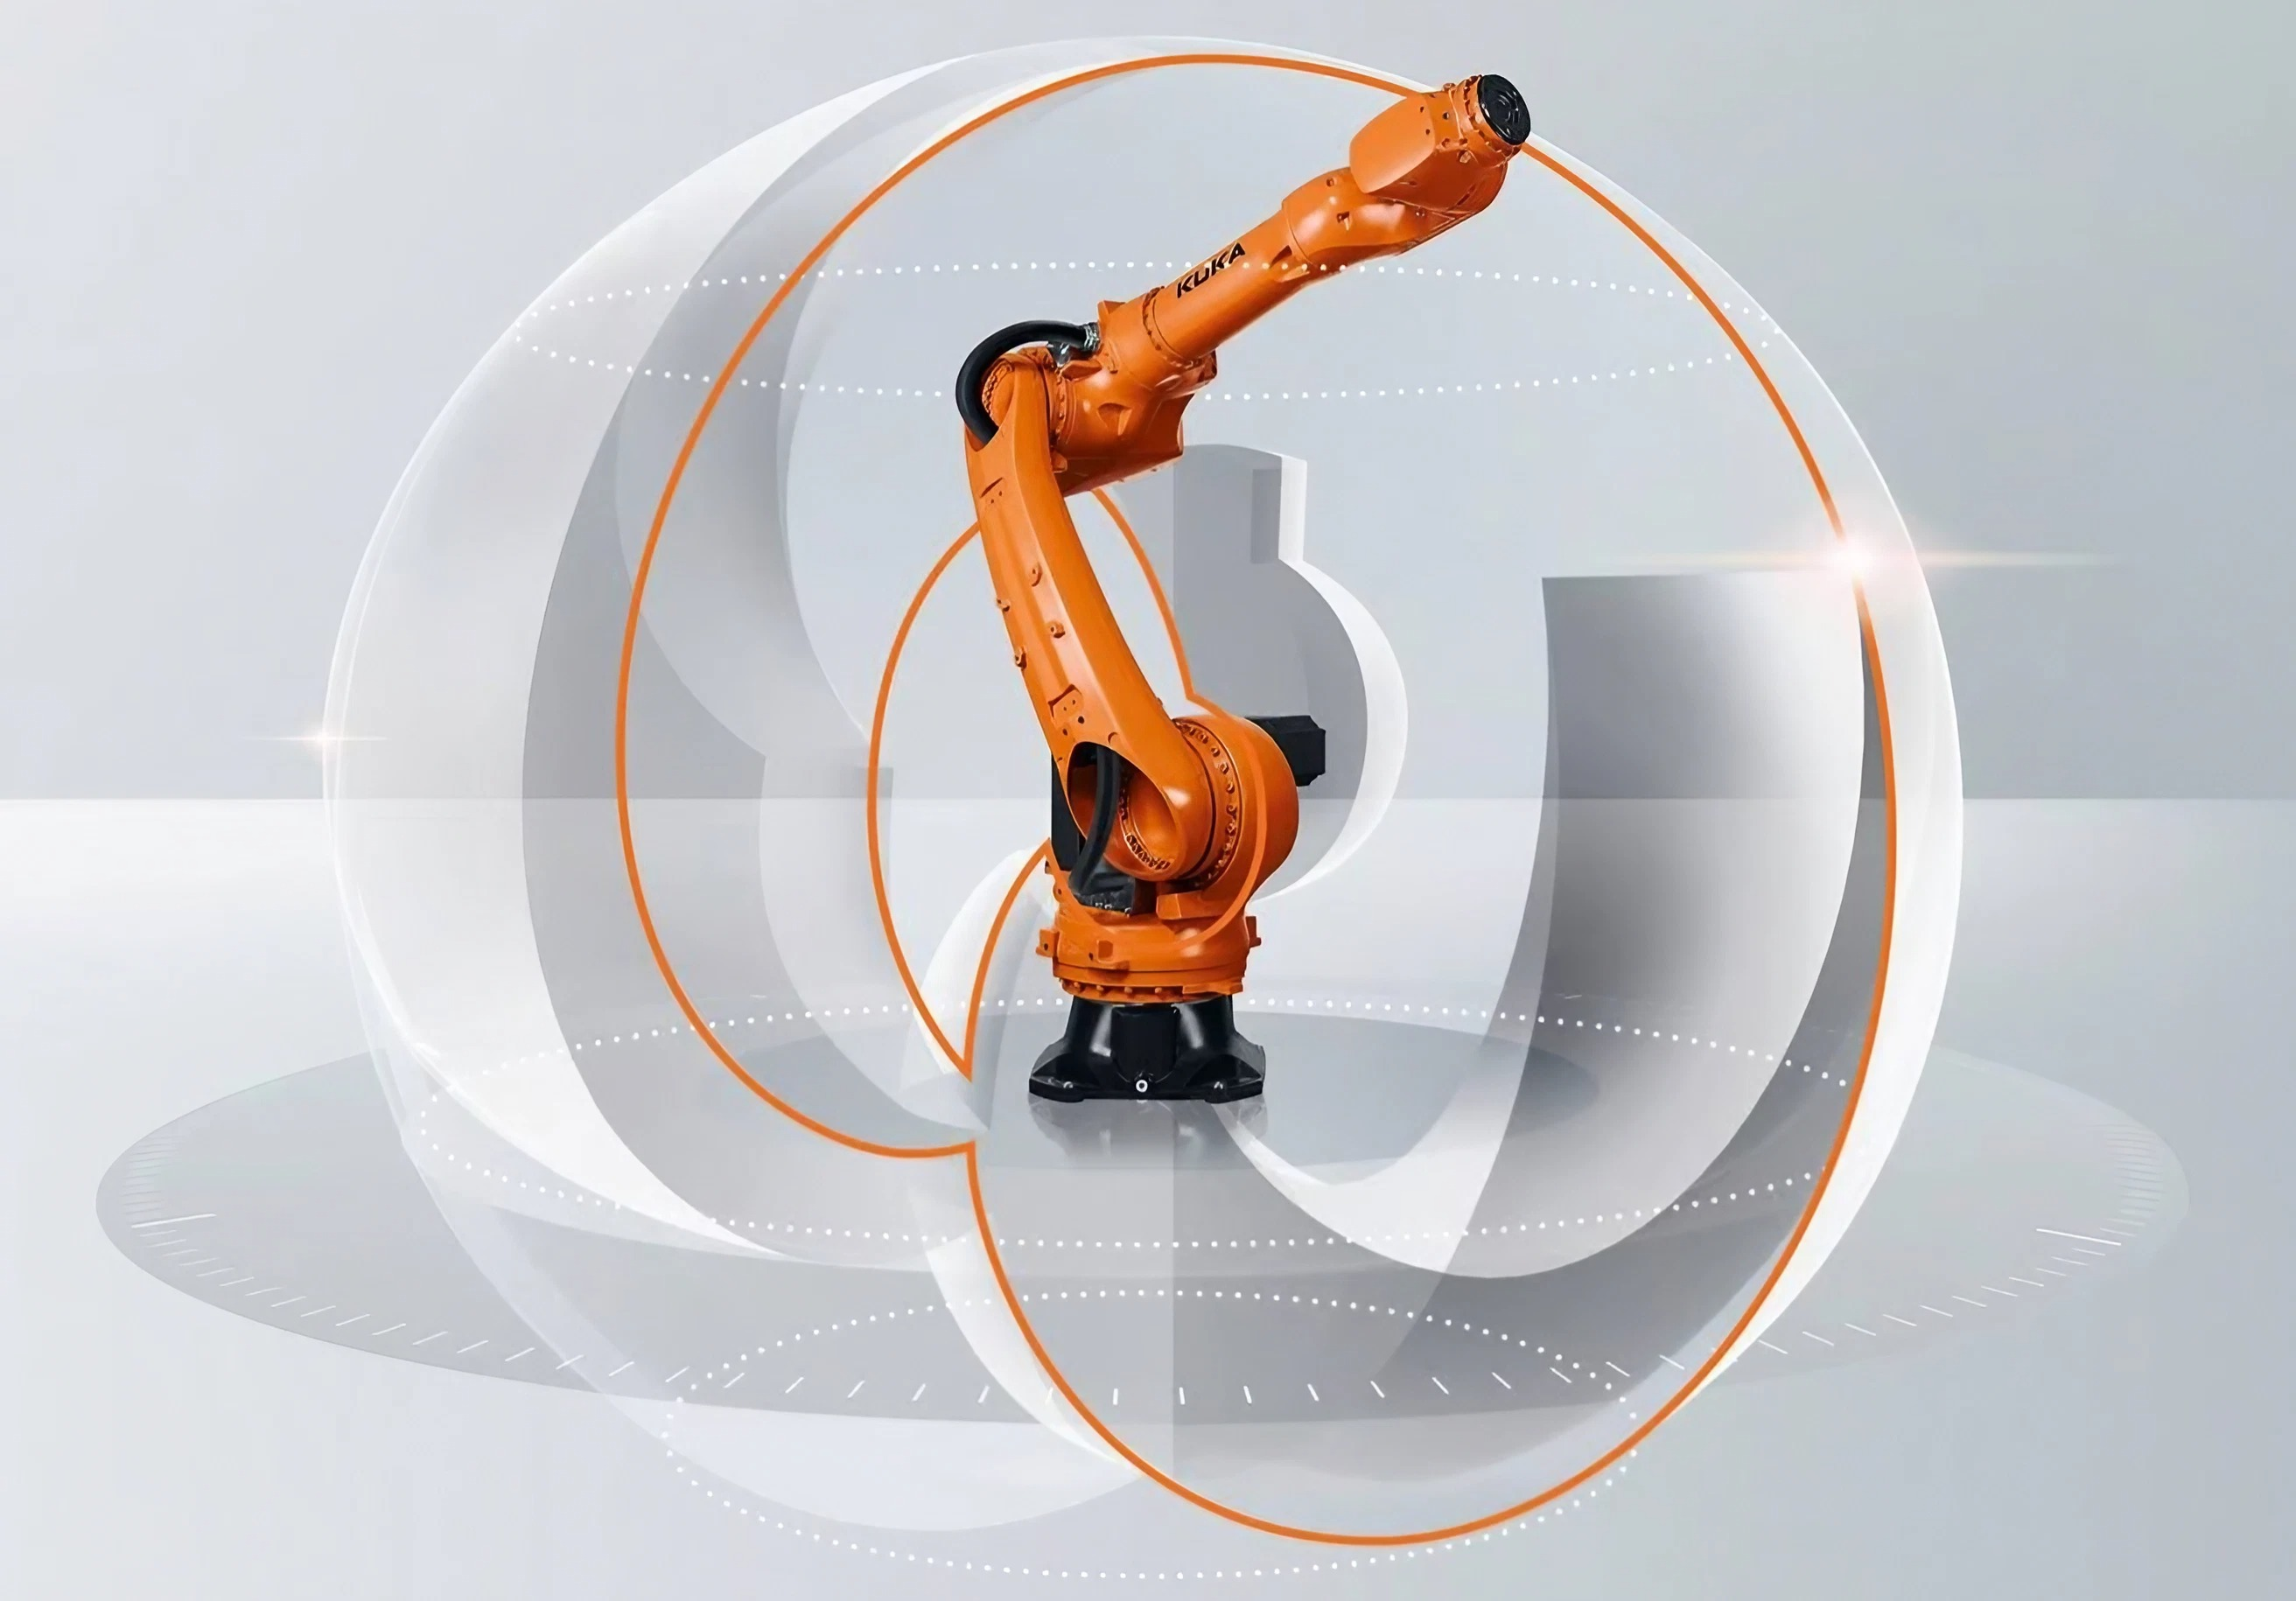
\includegraphics[width=0.4\linewidth ]{figs/kuka_articulado.jpg}}
  \hspace{1.5cm}
  \subfigure[ABB IRB 6700 \footnote{\url{https://new.abb.com/products/robotics/robots/articulated-robots/irb-6700}}]{\label{fig:irb6700}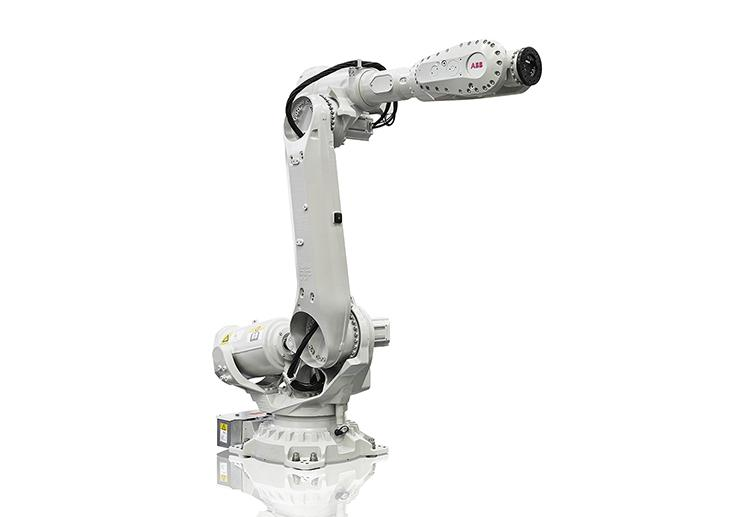
\includegraphics[width=0.4\linewidth]{figs/irb.jpg}}
  \caption{Robot articulados}
\end{figure}

\subsubsection{Paralelos}
\label{sec:paralelogramos}
Son un tipo de robot industrial que se caracteriza por tener una estructura mecánica en la cual varios brazos o cadenas cinemáticas se conectan de forma paralela a una plataforma móvil o 
base. Estos robots son rápidos y livianos, por lo que son ideales para aplicaciones que requieren alta velocidad, como en la industria alimentaria o en la selección y
empaquetado de productos.

\begin{figure} [ht!]
  \centering    
  \subfigure[Robot Delta ABB]{\label{fig:delta}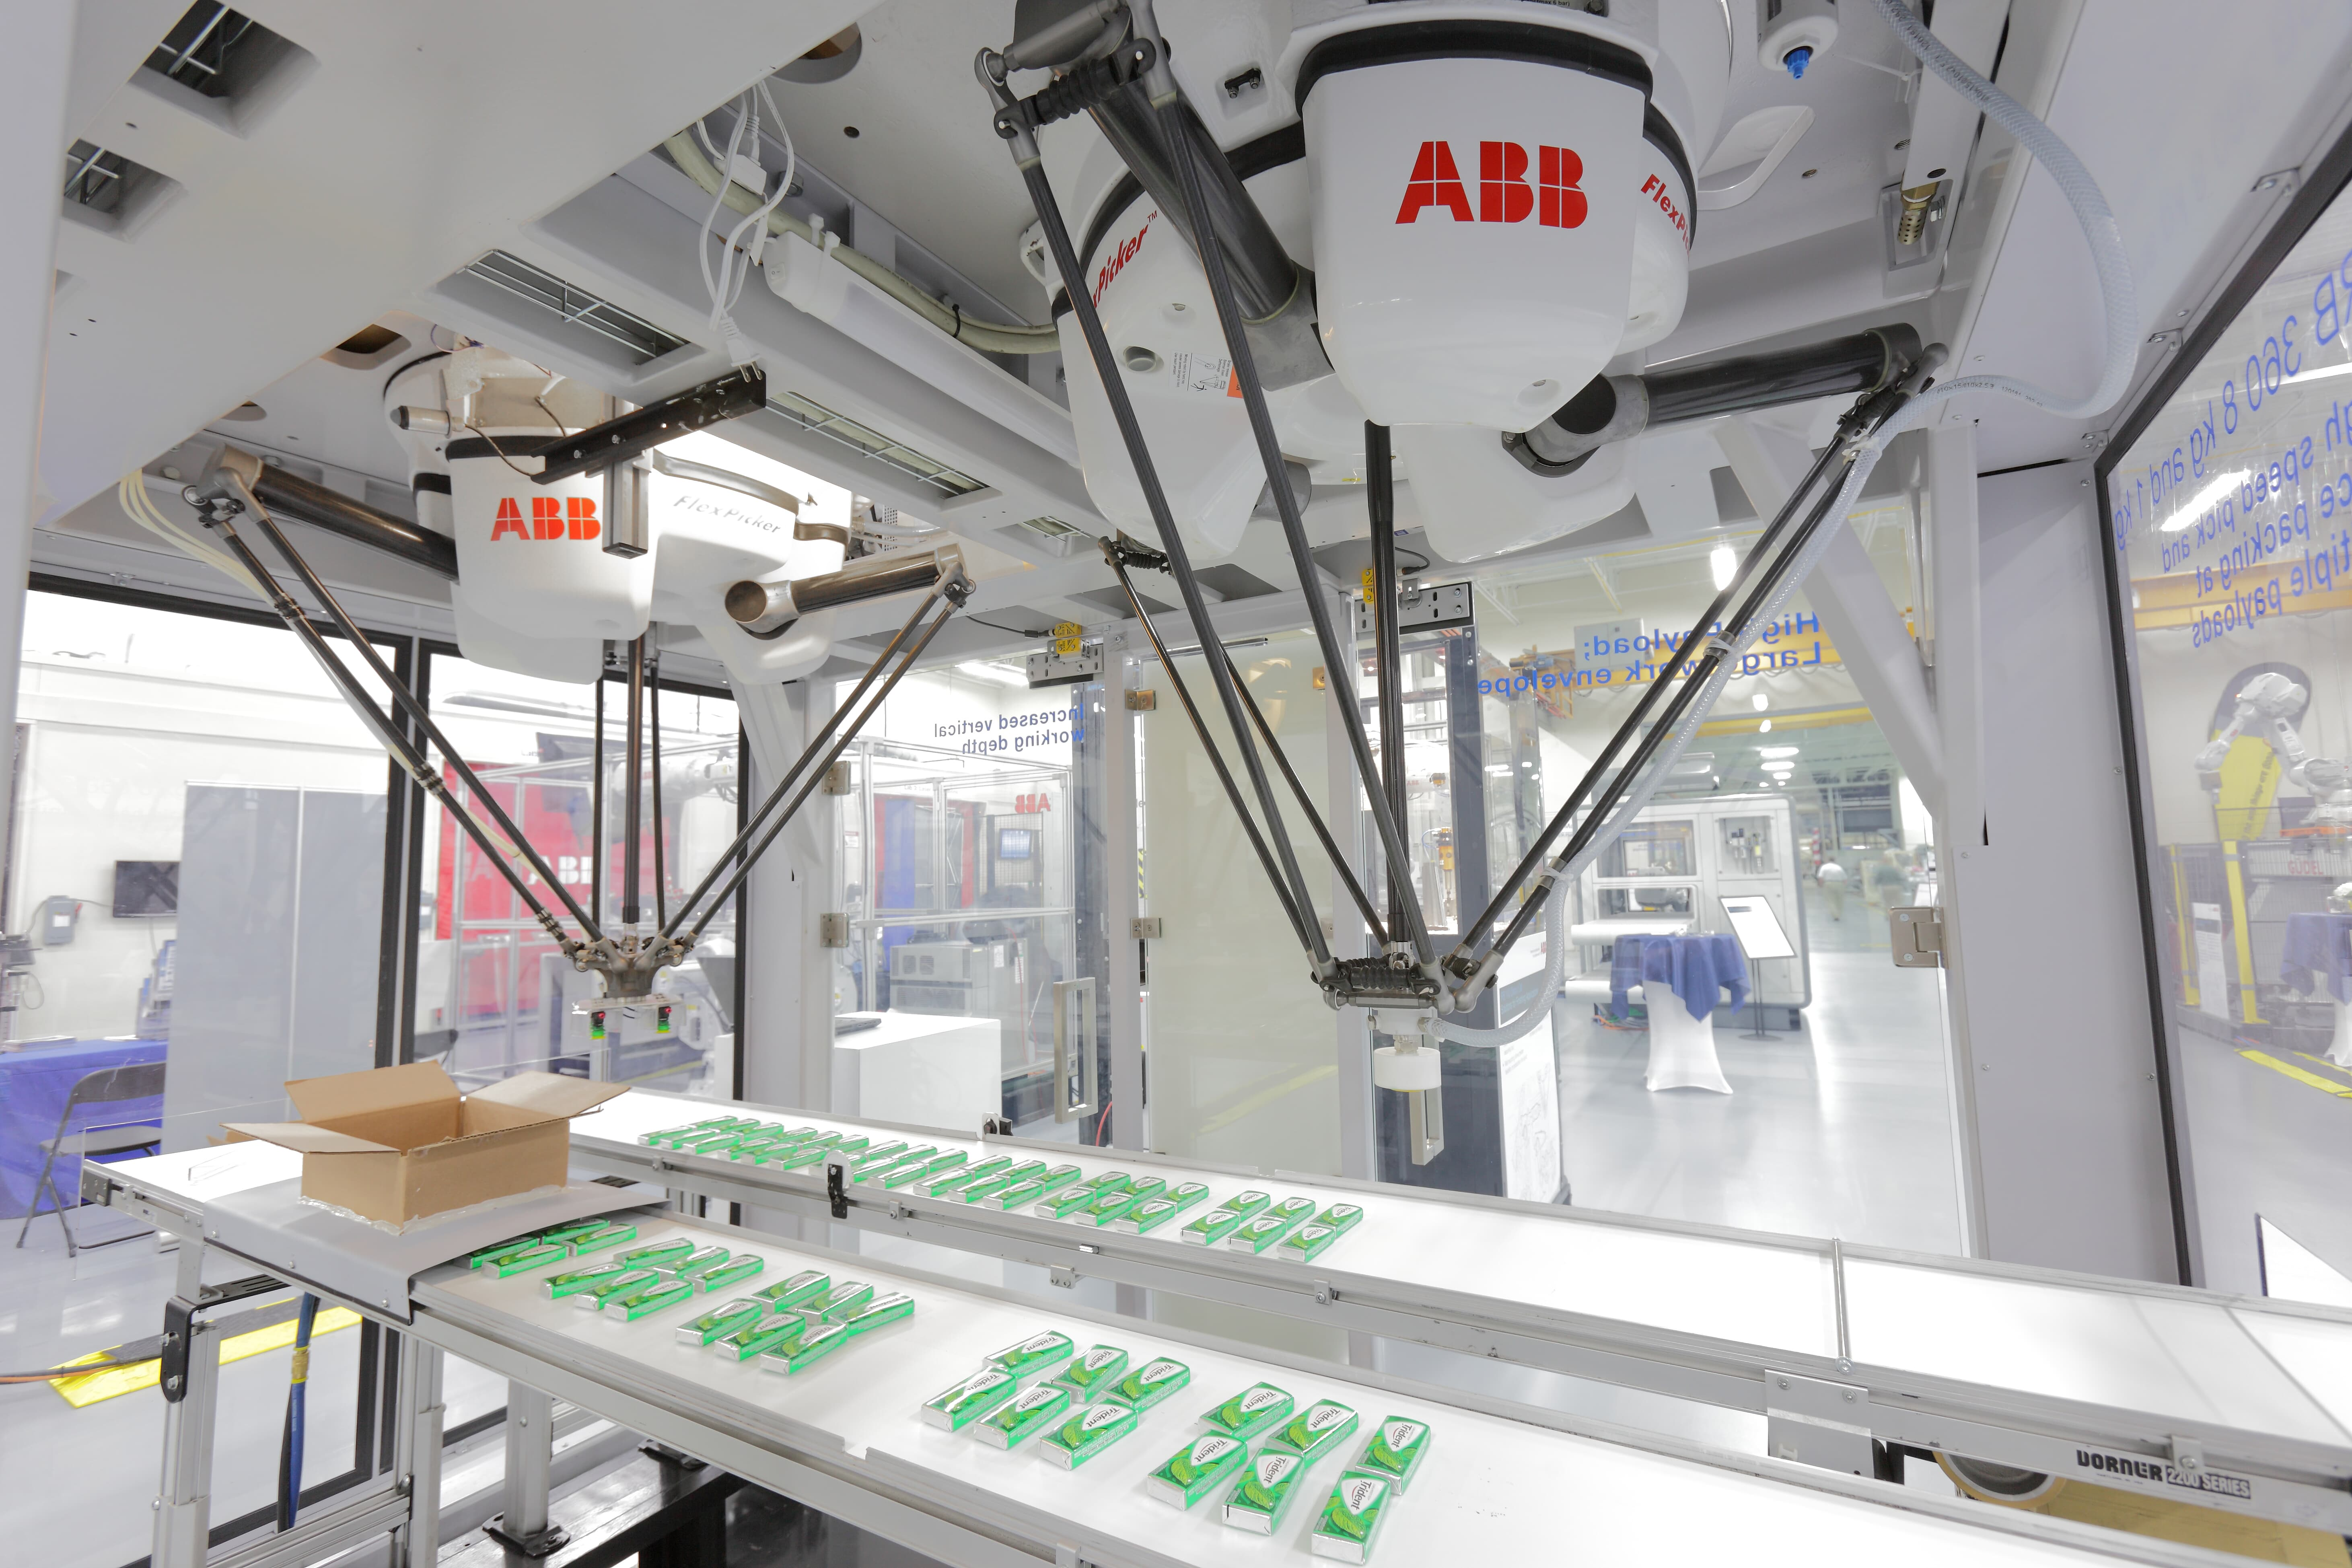
\includegraphics[width=0.4\linewidth ]{figs/delta_flex_picker.png}}
  \hspace{1cm}
  \subfigure[FANUC M-410iC]{\label{fig:paral}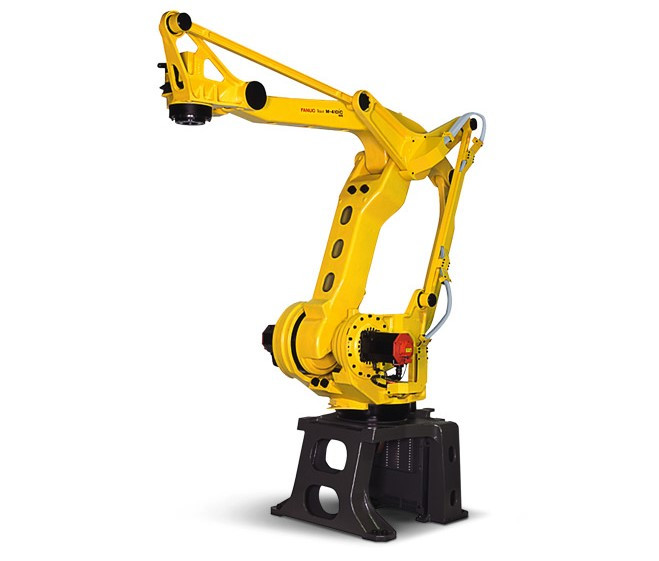
\includegraphics[width=0.4\linewidth]{figs/m_410.jpg}}
  \caption{Robots basados en paralelogramos}
\end{figure}

\newpage
\subsubsection{Cartesianos}
Los robots pertenecientes a esta categoría, se mueven a lo largo de unas guías lineales en la dirección de los tres ejes cartesianos (X, Y, Z) y cuyos ejes forman ángulos rectos entre sí. \\
Se trata de un tipo de máquina muy común en la industria y es usada en tareas de \textit{pick and place} y fresado, entre otras.

\begin{figure} [h!]
  \centering    
  \subfigure[VP-2500DP \footnote{\url{https://www.smallsmt.biz/bestueckungsautomat/}}]{\label{fig:pnp}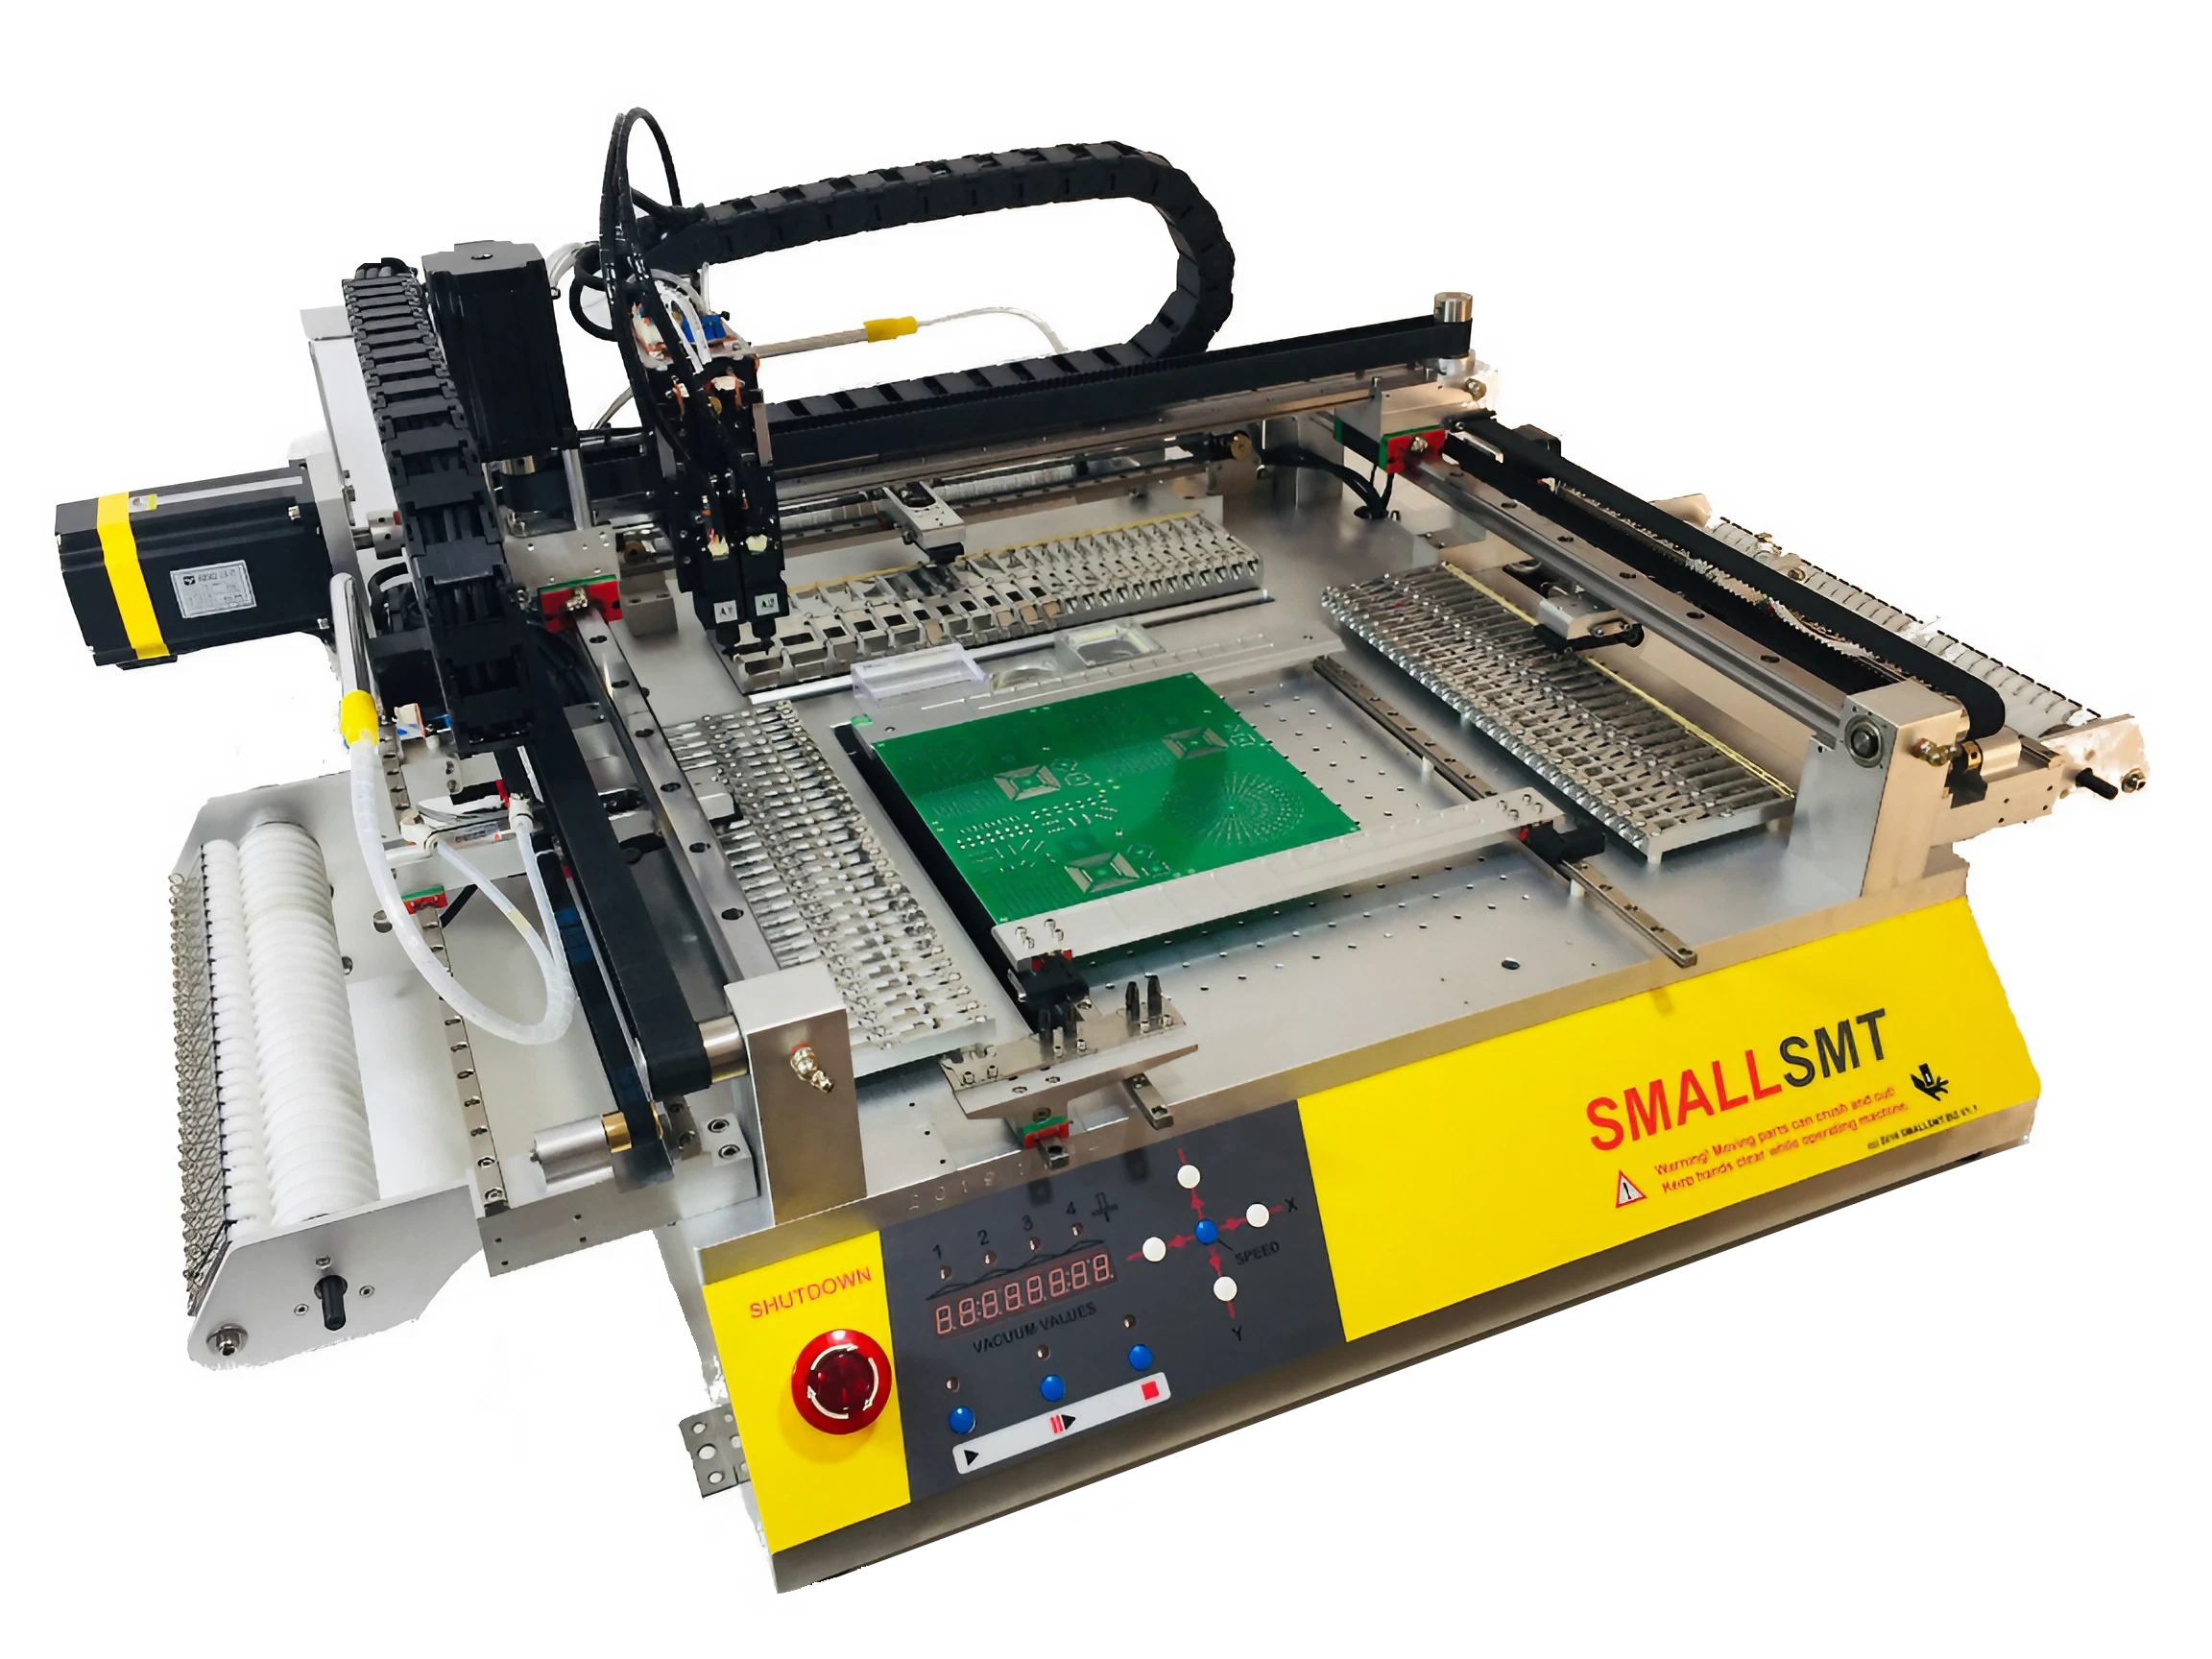
\includegraphics[width=0.4\linewidth ]{figs/pnp.jpg}}
  \hspace{1cm}
  \subfigure[OpenBuilds CNC Lead 1010 \footnote{\url{https://openbuilds.com/builds/lead-cnc-1010-40-x-40.7832/}}]{\label{fig:cnc}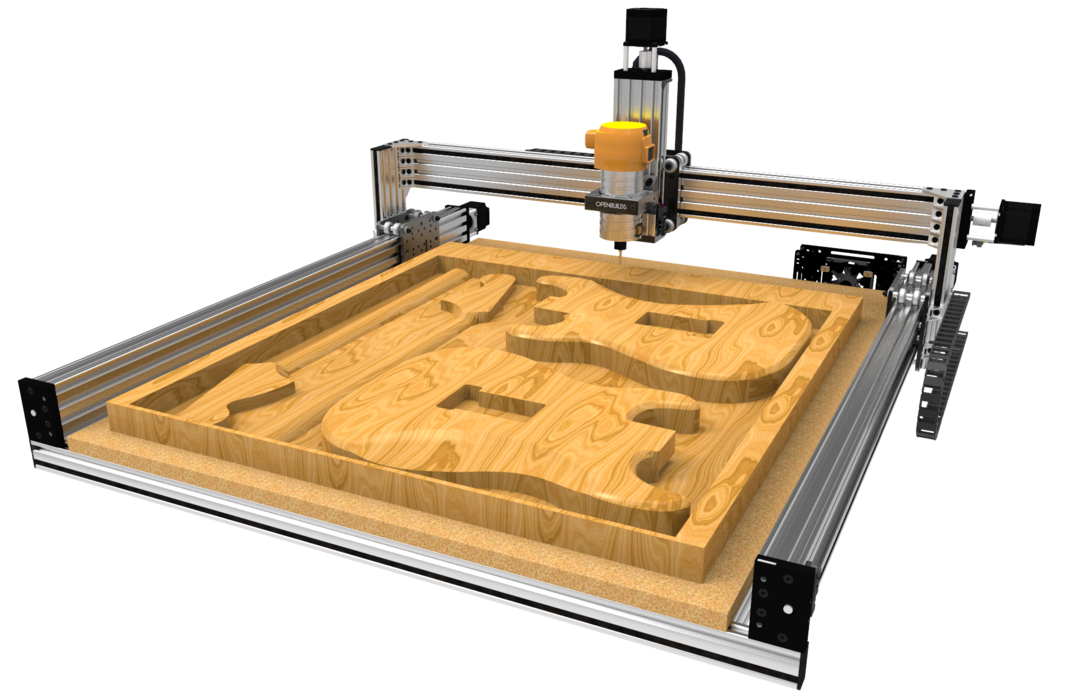
\includegraphics[width=0.4\linewidth]{figs/cnc.jpg}}
  \caption{Robots cartesianos}
\end{figure}

\section*{}
En resumen, la robótica es un campo en constante evolución que busca crear máquinas autónomas e inteligentes capaces de realizar una gran variedad de tareas cada vez 
más complejas. Sin embargo, a medida que la demanda de habilidades en robótica y automatización aumenta, se hace evidente la necesidad de formar a más personas en este campo.

\newpage
\section{Robótica educativa}
\label{sec:rob_educativa}
\noindent La robótica educativa es una disciplina que ha adquirido una gran relevancia en los últimos años debido a la creciente necesidad de formar a las nuevas generaciones en
competencias tecnológicas.
\subsection{Robótica en la educación secundaria}
\noindent En los institutos, la robótica se ha convertido en una herramienta pedagógica eficaz para desarrollar habilidades y conocimientos en áreas como la programación, 
la matemática, la electrónica y la resolución de problemas. Esto es conocido como \ac{STEM}. Gracias a esta formación, los 
estudiantes aprenden a diseñar, construir y programar robots simples para llevar a cabo una tarea específica, lo que les ayuda a comprender  
los conceptos de ciencia y tecnología de una manera más práctica e interactiva.\\
\begin{figure} [ht!]
  \centering    
  \subfigure[Instituto en Argentina \footnote{\url{https://www.diariodecuyo.com.ar/suplementos/Robotica-la-ciencia-de-aprender-jugando-20170907-0087.html}}]{\label{fig:instituto_sanjuan}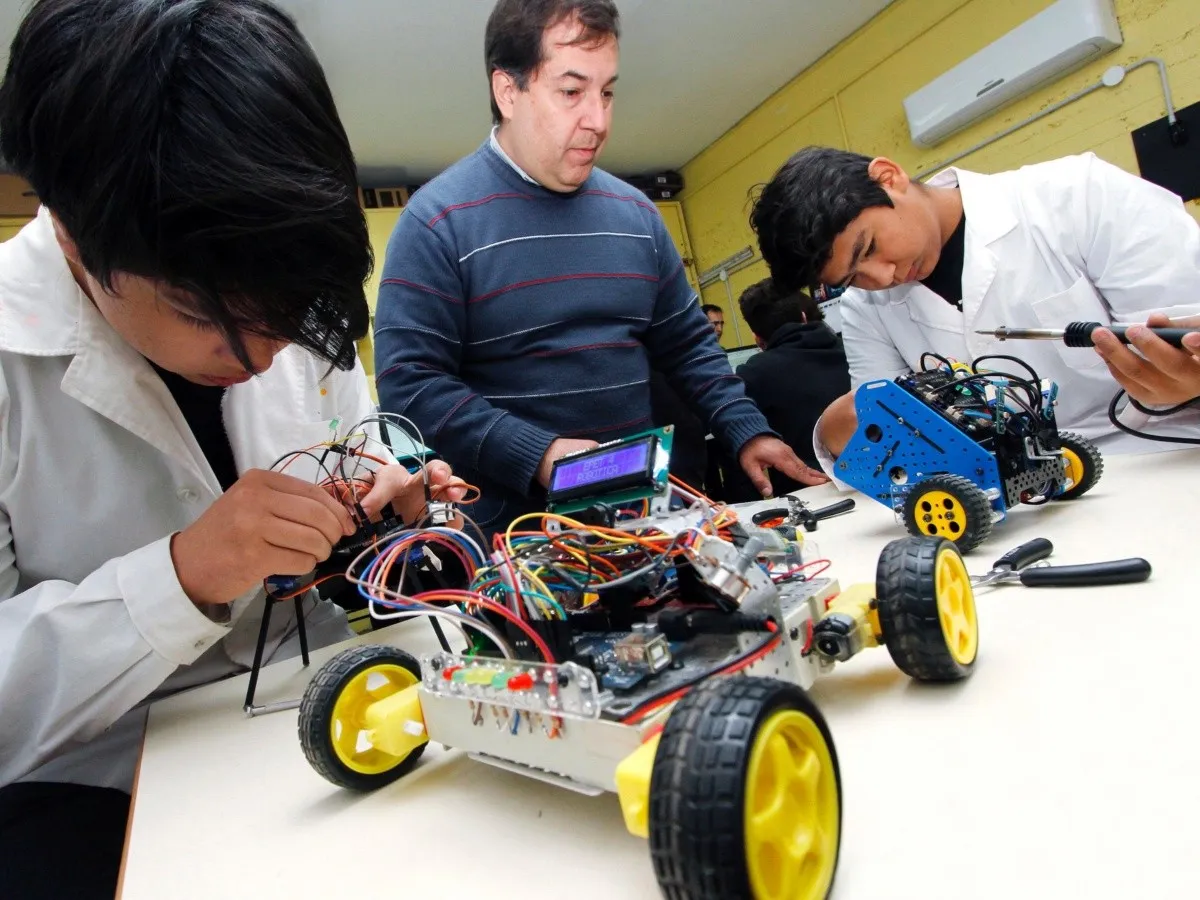
\includegraphics[width=0.4\linewidth ]{figs/robots_instituto.jpg}}
  \hspace{1cm}
  \subfigure[Institutos en Toledo \footnote{\url{https://www.uclmtv.uclm.es/institutos-de-camarena-y-madridejos-ganan-el-viii-torneo-de-robotica-organizado-por-la-uclm-en-toledo/}}]{\label{fig:instituto_toledo}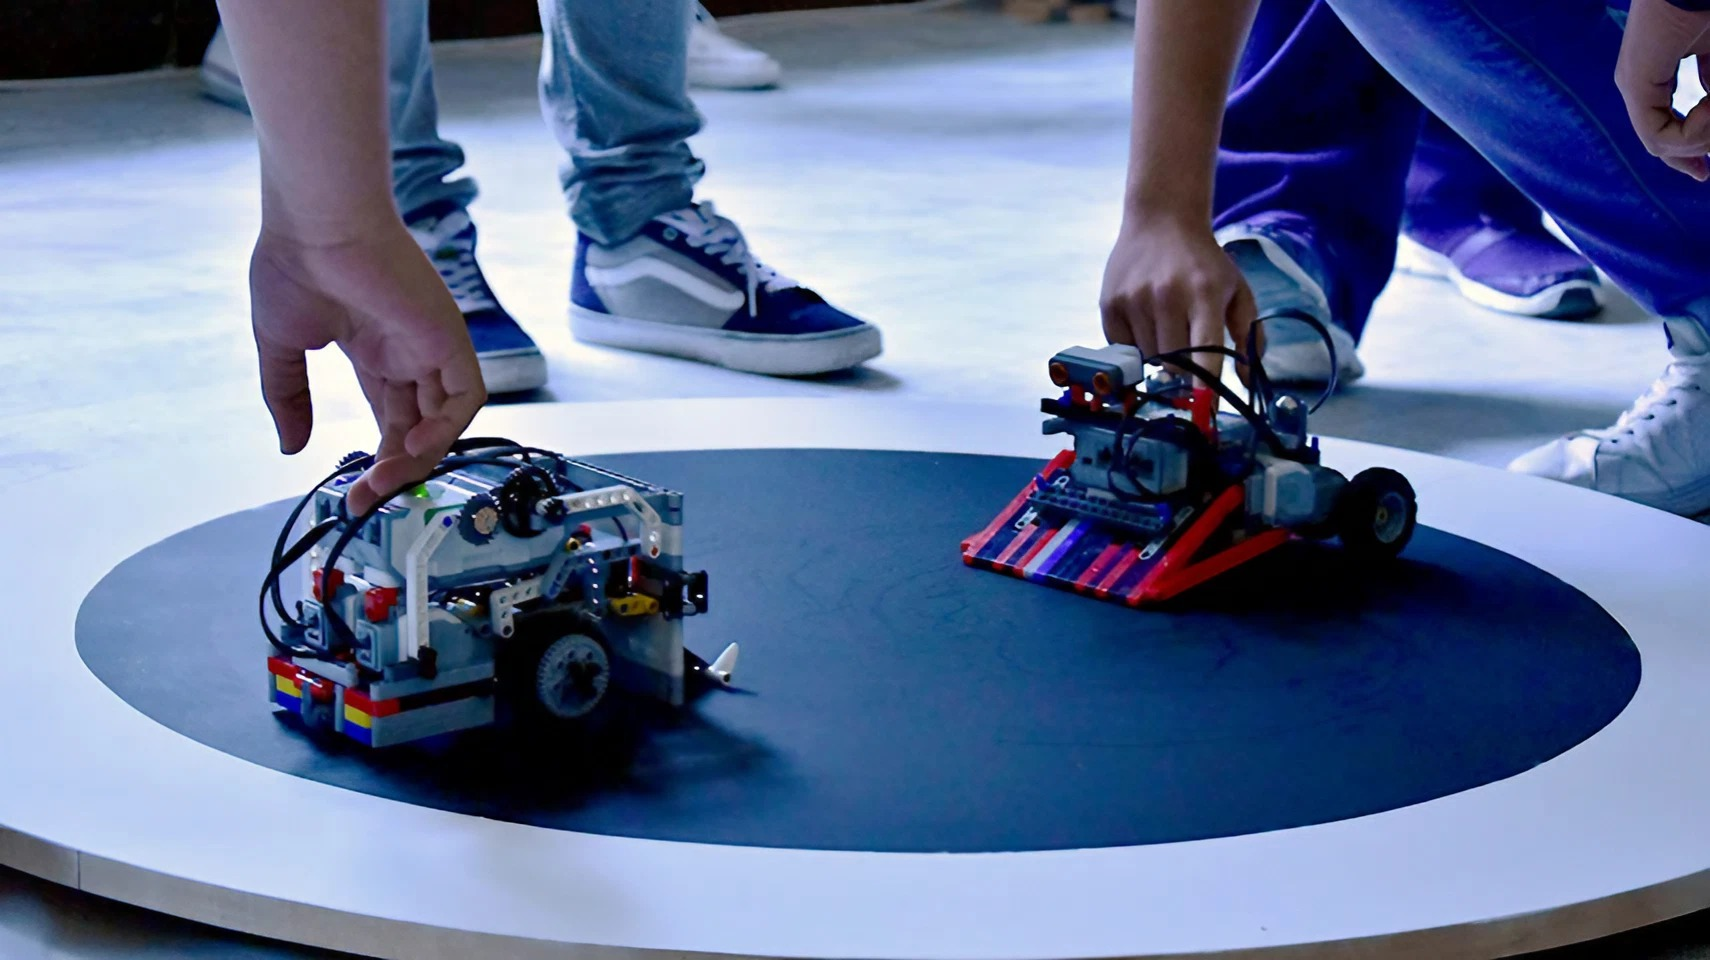
\includegraphics[width=0.5\linewidth]{figs/robot_batalla_instituto.jpg}}
  \caption{Robots en institutos}
\end{figure}

\newpage
\subsection{Robótica en la universidad}
\noindent A nivel universitario, la robótica se ha convertido en una disciplina esencial para formar a los futuros ingenieros. Los estudiantes aprenden 
a diseñar y construir robots más avanzados, y refuerzan sus habilidades de programación y control de sistemas complejos. En estos centros 
se hace uso de varios tipos de robots, como pueden ser, brazos industriales y plataformas robóticas móviles como los mostrados en la Figura \ref{fig:robots_universidades}. Al tratarse de sistemas 
usados en el mundo profesional, los estudiantes pueden aprender con robots similares a los que usarán en un futuro. 

\begin{figure} [ht!]
  \centering    
  \subfigure[Turtlebot 2 \footnote{\url{https://www.turtlebot.com/turtlebot2/}}]{\label{fig:turtlebot}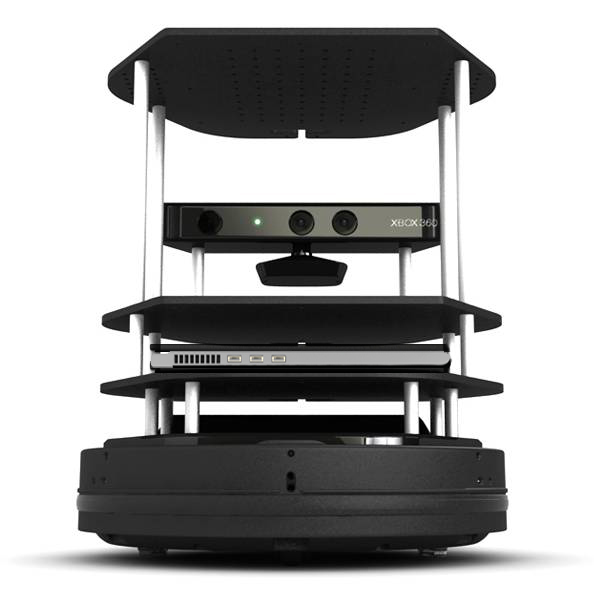
\includegraphics[width=0.28\linewidth ]{figs/turtlebot.jpg}}
  \hspace{1cm}
  \subfigure[Dobot Magician \footnote{\url{https://www.robotlab.com/store/dobot-robotic-arm}}]{\label{fig:dobot}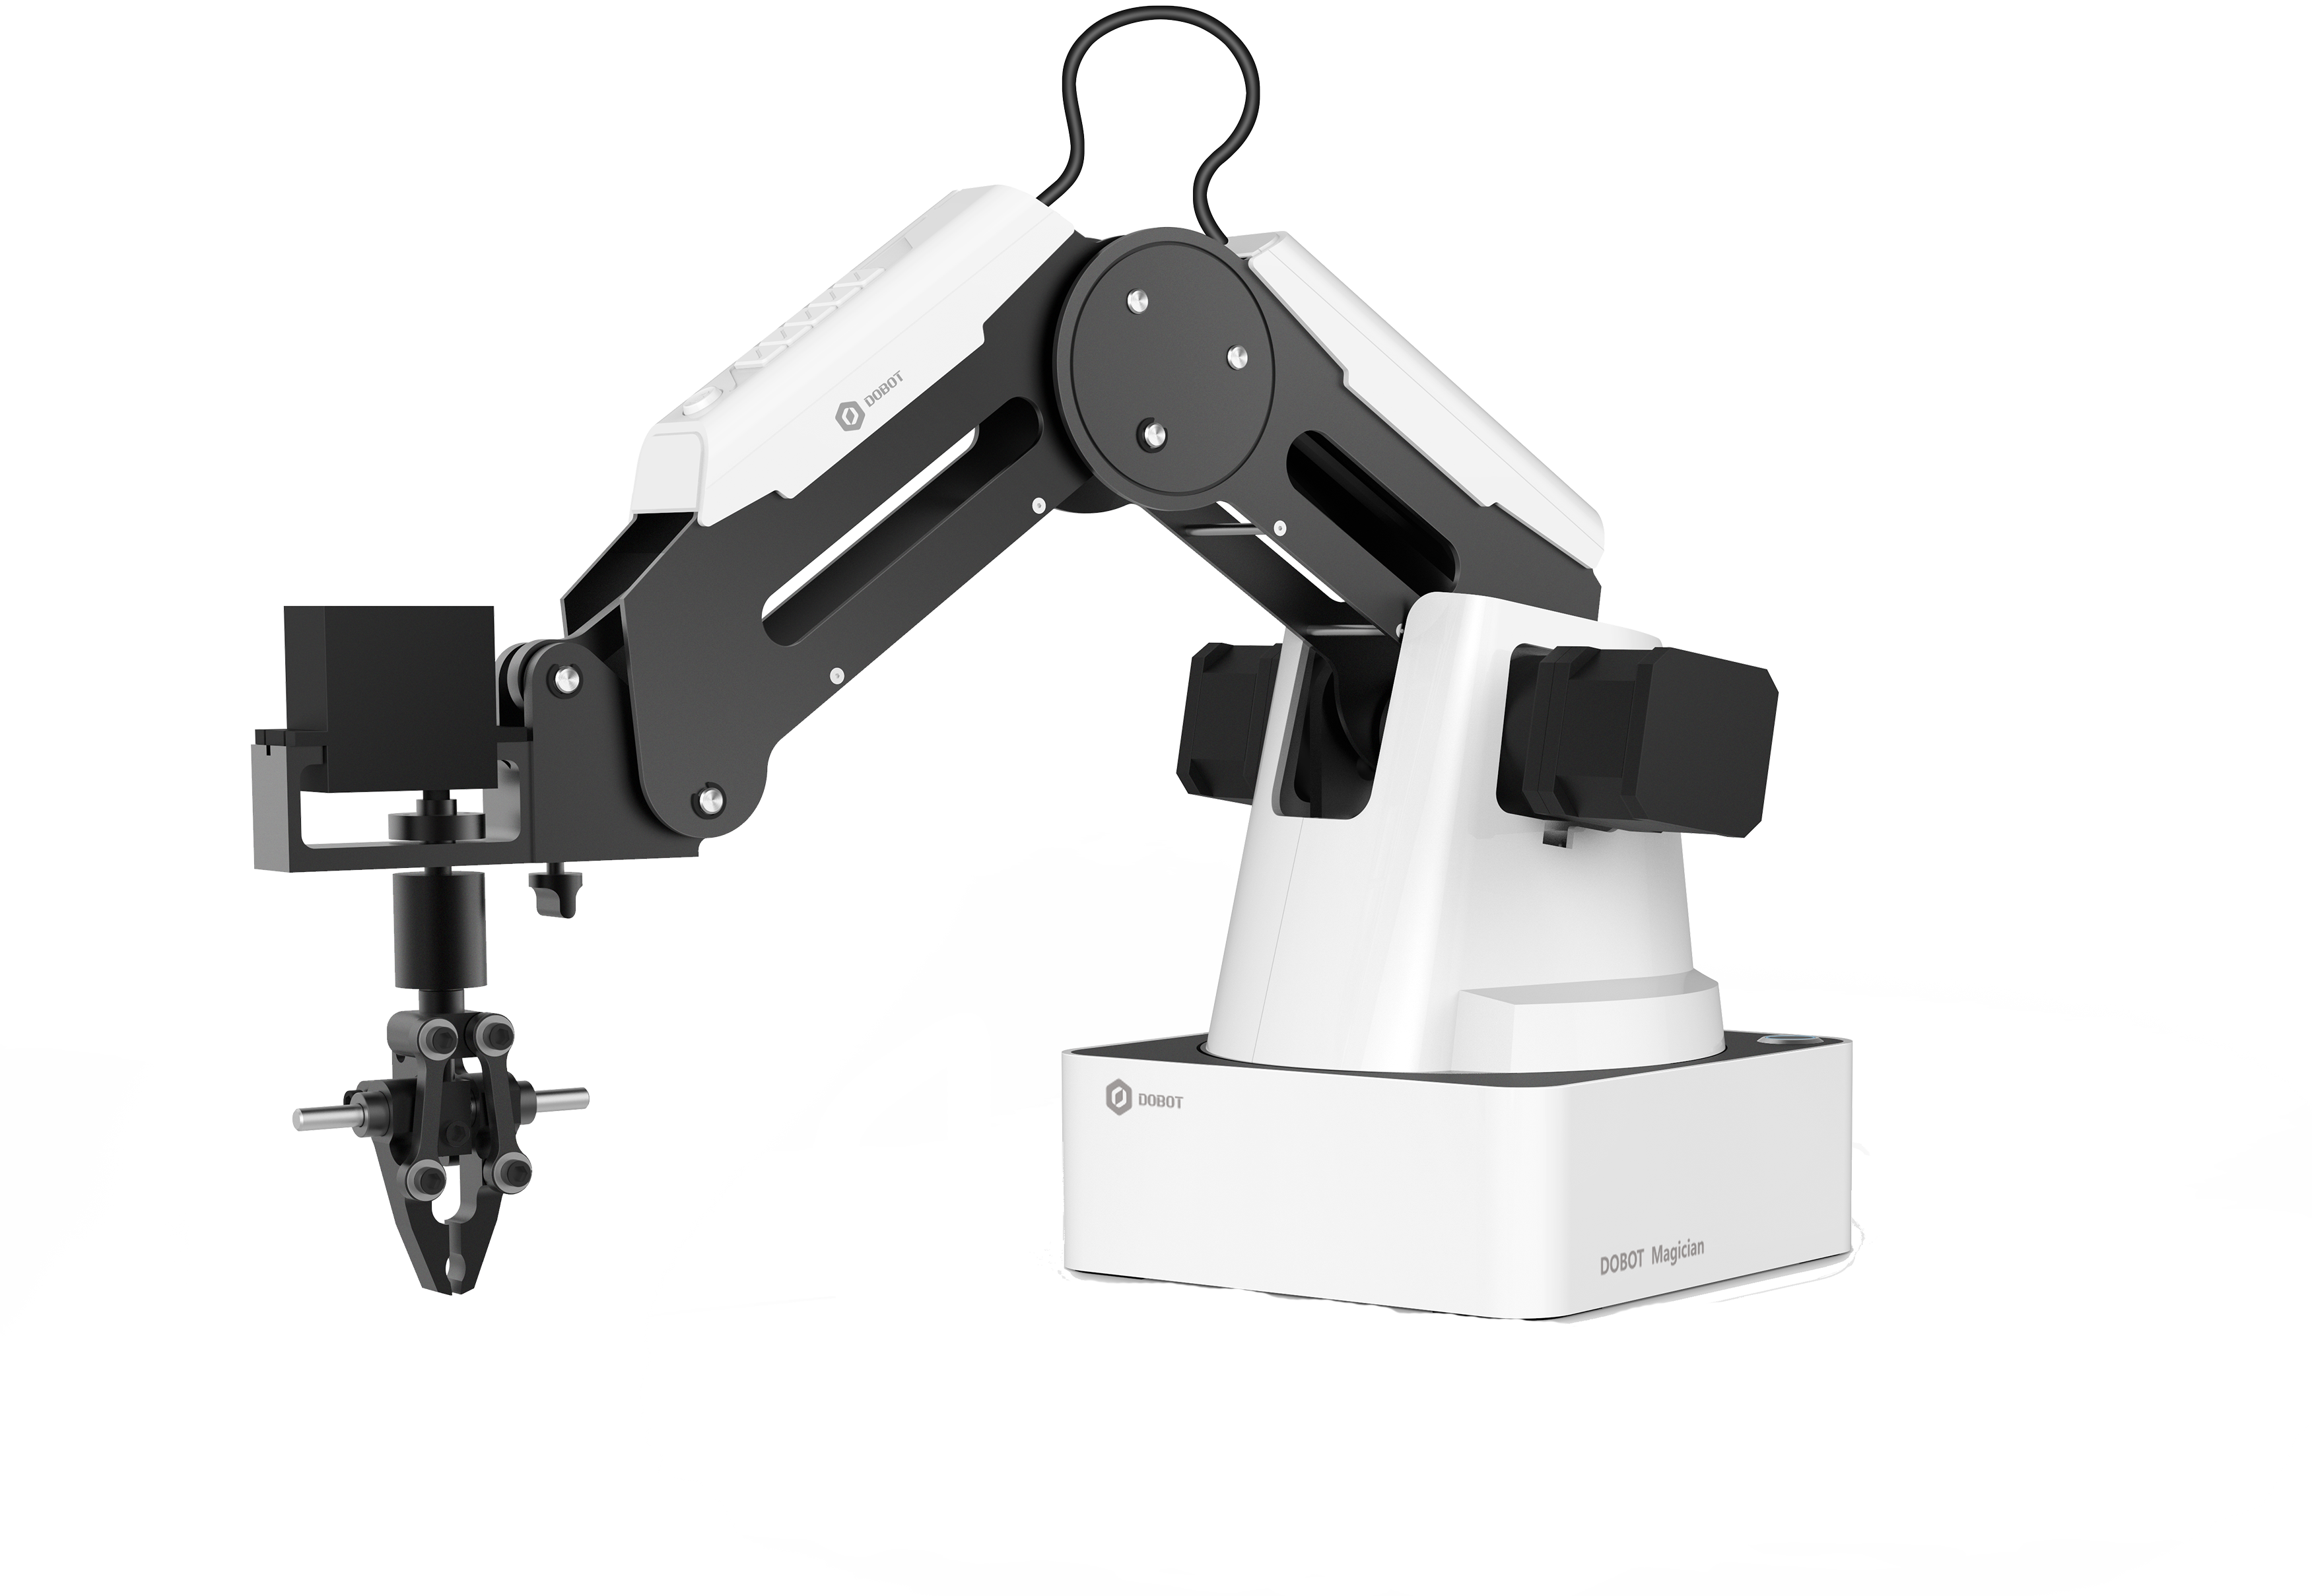
\includegraphics[width=0.36\linewidth]{figs/dobot.png}}
  \subfigure[UR3e \footnote{\url{https://www.universal-robots.com/es/productos/robot-ur3/}}]{\label{fig:ur3e}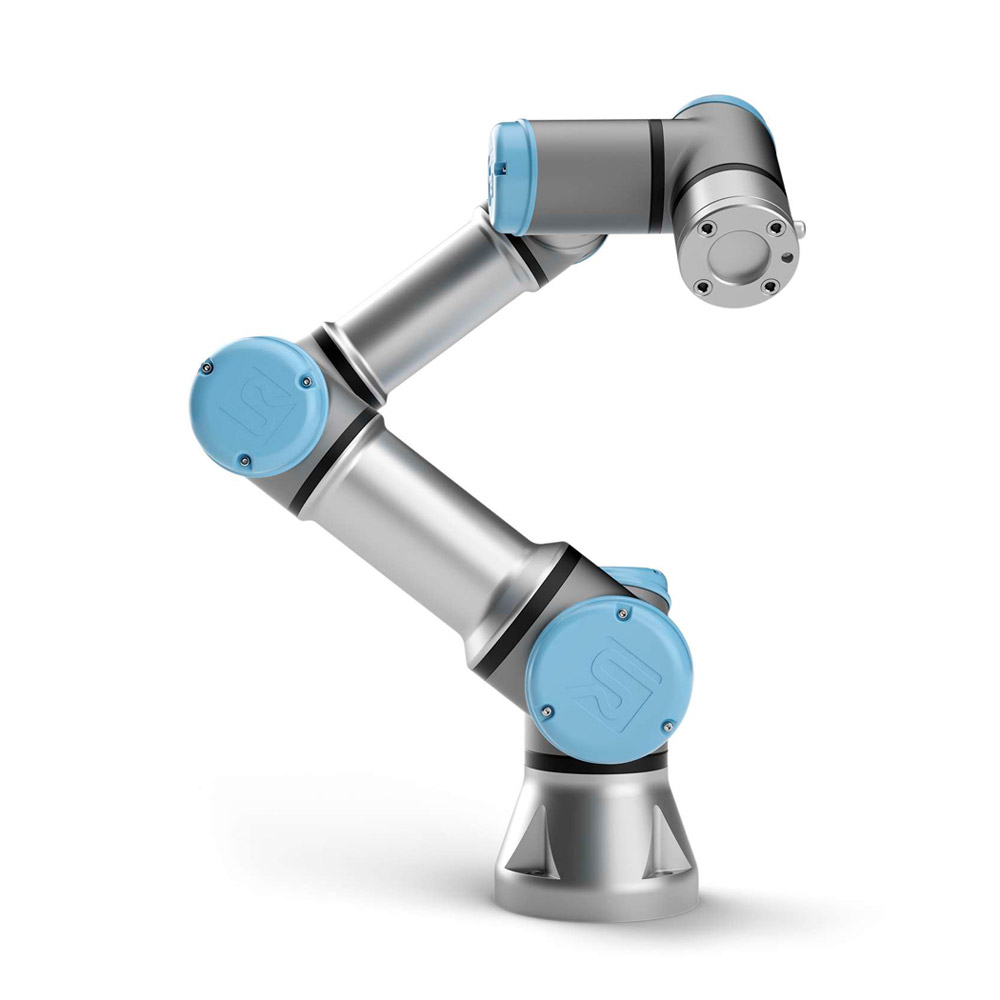
\includegraphics[width=0.27\linewidth]{figs/UR3e.jpg}}
  \caption{Robots usados en universidades}
  \label{fig:robots_universidades}
\end{figure}

Por contra, aunque es verdad que las universidades disponen de algunas unidades, no siempre son accesibles para el 
estudiante por diversas razones. La mayor de ellas es su elevado coste que reduce la cantidad de unidades que se puede 
permitir la universidad. Es por esto que existe la creciente necesidad de crear robots asequibles para su uso en enseñanza.

\newpage
\section{Robótica de bajo coste}
\label{sec:rob_bajo:coste}
\noindent La robótica de bajo coste es el área de la robótica enfocada en el diseño y desarrollo de robots 
accesibles y asequibles. Tiene como objetivo conseguir desarrollar tecnología robótica
barata, reduciendo la complejidad de los sistemas empleados y haciendo uso de materiales más económicos.

La disponibilidad de herramientas de fabricación de bajo coste, como la impresión 3D y el corte láser, 
ha hecho posible que los usuarios puedan crear piezas y componentes robóticos personalizados a un 
precio más bajo que el de la fabricación tradicional.

En este campo de la robótica se hace patente la Ley de Moore, una ley teórica 
que establece que la capacidad de procesamiento de los microchips se duplica cada dos años. Esta observación, que 
se planteó hace casi 60 años, sigue siendo válida en la actualidad y ha sido fundamental para el desarrollo de componentes 
electrónicos cada vez más pequeños, eficientes y potentes. Gracias a esto, ha surgido la filosofía del \enquote{Hazlo tú mismo} o \ac{DIY}, que se enfoca en la creación de proyectos personalizados y 
asequibles utilizando tecnología de bajo coste y materiales comunes.

En resumen, la robótica de bajo coste es una consecuencia directa del crecimiento de la capacidad de computación, 
el abaratamiento de los precios de los componentes electrónicos y el enfoque \acs{DIY}.
El desarrollo de esta tecnología, permite que más personas puedan experimentar en este área de la ingeniería y desarrollar 
sus propias soluciones robóticas.
\begin{figure} [ht!]
  \centering    
  \subfigure[OSTR \footnote{\url{https://www.instructables.com/Low-Cost-Arduino-Compatible-Drawing-Robot/}}]{\label{fig:osrt}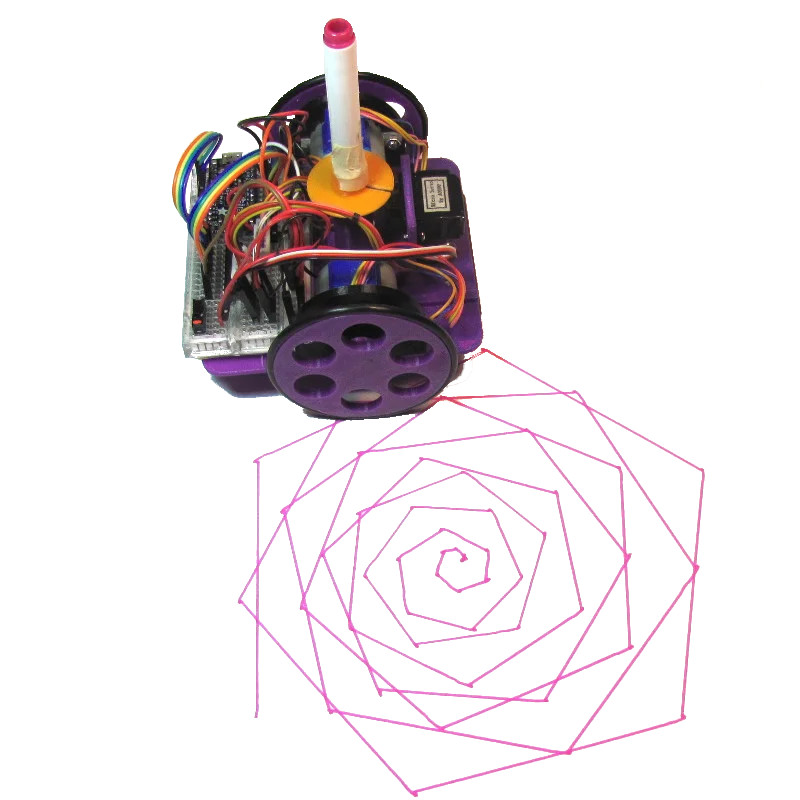
\includegraphics[width=0.35\linewidth ]{figs/OSTR.jpg}}
  \hspace{1cm}
  \subfigure[Diy-robotics 6-DOF \footnote{\url{https://diy-robotics.com/educative-robot-cell-free-package/?utm_source=Instructables.com&utm_medium=referrer&utm_campaign=Educative\%20Cell}}]{\label{fig:diyrobotics}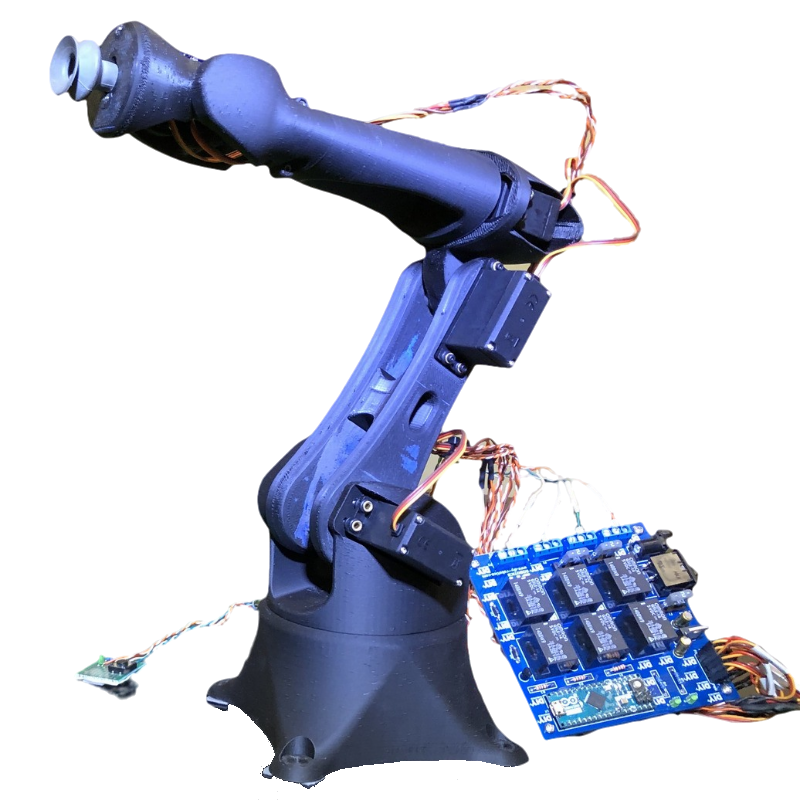
\includegraphics[width=0.35\linewidth]{figs/diyroboticsarm.png}}
  \caption{Robots de bajo coste}
\end{figure}
